\documentclass[12pt,a4paper]{book}
\usepackage[utf8]{inputenc}
\usepackage[margin=1in]{geometry}
\usepackage{titling}

% Images
\usepackage{graphics}
\graphicspath{ {img/} }
\usepackage{svg}

% Automatically match quotation marks
\usepackage{csquotes}
\MakeOuterQuote{"}

% Bibleography
\usepackage[backend=biber]{biblatex}
\addbibresource{Dissertation.bib}

% Indent first paragraphs in sections and chapters
\usepackage{indentfirst}

% Graphical Models
\usepackage{tikz}
\usetikzlibrary{fit,positioning,bayesnet}
\usetikzlibrary{arrows}
% Layer separation for neural network figure
\def\layersep{2.5cm}

% Indent description lists
\usepackage{enumitem}
\setlist[description]{leftmargin=\parindent,labelindent=\parindent}

\usepackage{amsmath}
\usepackage{amsfonts}
% Use full stop for comma
\mathchardef\period=\mathcode`.
\DeclareMathSymbol{.}{\mathord}{letters}{"3B}

% Additional information for figures
\usepackage{caption}

%Tables
\usepackage{makecell, array, booktabs}
\renewcommand\theadfont{\bfseries}


% New commands
\newcommand\college{Clare College}
\newcommand\mean[1]{\overline{#1}}
\newcommand\bs[1]{\boldsymbol{#1}}
\newcommand\note[1]{\vspace*{-0.5\baselineskip}\caption*{#1}}


% Display JSON nicely
\usepackage{xcolor}
\usepackage{minted}
%% fix the minted@colorbg environment
\makeatletter
\renewenvironment{minted@colorbg}[1]
 {\def\minted@bgcol{#1}%
  \noindent
  \begin{lrbox}{\minted@bgbox}
  \begin{minipage}{\linewidth-2\fboxsep}}
 {\end{minipage}%
  \end{lrbox}%
  \setlength{\topsep}{\bigskipamount}% set the vertical space
  \trivlist\item\relax % ensure going to a new line
  \colorbox{\minted@bgcol}{\usebox{\minted@bgbox}}%
  \endtrivlist % close the trivlist
 }
\makeatother



\title{Predicting statistical results in competitive computer games}
\author{Artem Vasenin}
\date{\today}



\begin{document}
\frontmatter


\pagestyle{empty}

\rightline{\LARGE \textbf{\theauthor}}

\vspace*{60mm}
\begin{center}
\Huge
\textbf{Predicting statistical results in competitive computer games} \\[5mm]
Computer Science Tripos -- Part II \\[5mm]
\college \\[5mm]
\today  % today's date
\end{center}



\cleardoublepage
\pagestyle{plain}

\section*{Proforma}
\begin{description}
\item[Name] \theauthor
\item[College] \college
\item[Title] Predicting statistical results in competitive computer games.
\item[Examination] Computer Science Tripos -- Part II, June 2017
\item[Word Count] 9336\footnote{Calculated using \mintinline{bash}{pdftotext Disseration.pdf -f 9 -l 42  - | wc -w}.} %TODO
\item[Project Originator] Artem Vasenin (av429)
\item[Project Supervisor] Yingzhen Li (yl494)
\end{description}

\subsection*{Original Project Aim}
The aim of this project was to develop an algorithm which could predict whether certain events would happen in multiplayer computer games.
In most modern multiplayer games, players are provided with a summary after each match describing their performance in that match and outlining key choices they have made.
The project should be able to predict the values present in such summary.
The mean squared error of such predictions should be less than half of variance of the variable.
\subsection*{Summary of Work Completed}
A graphical model was created which produces a probability distribution for continuous variables.
The first prototype was built using a combination of ad-hoc use of TrueSkill and machine learning functions from scikit-learn python library.
The final version was created entirely using TensorFlow and Keras.
The system achieved $R^2$ value of more than 0.5 on one variable in the dataset and over 0.25 on another three.
\subsection*{Special Difficulties}
There was a mistake in the project proposal success criteria, which is explained in section \ref{requirements-error}.


\section*{Declaration of Originality}
I, \theauthor\ of \college, being a candidate for Part II of the Computer Science Tripos, hereby declare that this dissertation and the work described in it are my own work, unaided except as may be specified below, and that the dissertation does not contain material that has already been used to any substantial extent for a comparable purpose. % This is one long-ass sentense
\\[1\baselineskip]
\noindent Signed 
\\[1\baselineskip]
\noindent Date: \thedate

\section*{Acknowledgements}
I would like to thank my supervisor, Yingzhen Li, for the weekly meetings throughout the project's duration and helping me understand the complex methods used in modern machine learning approaches.

\clearpage
\tableofcontents
\listoffigures

\mainmatter
\chapter{Introduction}
\section{Motivation}
Multiplayer computer games are becoming very popular, more than a 100 million people play League of Legends every month \cite{league100}.
A game's success often rests on how enjoyable it is.
Current method of improving player experience is to make sure that all players have equal chance of winning a match.
For that purpose their skill has to be tracked and teams have to be arranged such that they are of equal strength.

In many popular games several roles have to be filled on each team for optimal performance.
Current algorithms, such as TrueSkill \cite{trueskill}, only track player's overall skill and do not consider what roles the player prefers and how good they are at each one.
This often leads to teams being composed of players all wanting to play the same role, which either leads to team under-performing or some players not enjoying the game as much as they could.
Moreover, I believe that the events that happen in a match are more important to many player's experience than the actual outcome.

To be able to match players better, a system has to be built that will take into account how the game is played and what strategies exist in it.
Creating such a system using classical techniques would require deep knowledge of workings of the game.
Unfortunately, I do not have such knowledge of most games and obtaining such knowledge although might be fun, will take too long and will be inefficient.
Furthermore, most such games change their rules every few months to keep players interested, therefore performance of hard coded system would decrease as the time goes on.
As a result I decided to use machine learning techniques which would help me create a system which can adapt to different games by itself and also update its judgement as game changes.

\section{Related Work}
Before starting the project, I have looked into papers and articles about predicting events in sports and computer games.
I have found out that nothing similar has been done before.
Most closely related algorithms (such as \cite{trueskill} and \cite{bayesianranking}) were made to only predict the outcome of a match , not any related results.
Outside of academia, other algorithms were made which used machine learning to improve their performance, but again only focusing on the outcome of a match.
%TODO Write more here


\chapter{Preparation}
\section{Proposal Refinement}
I had two drafts of my project proposal, this being my first major project I had little experience in preparing a plan.
After receiving comments from my overseers regarding the first draft of the proposal, I have incorporated several changes in the project proposal, including:
\begin{itemize}
\item Add a time-line, deadlines and deliverables to the project plan, to be able to track the progress of the project accurately.
\item Limited and listed all of the potential variables that will be considered, to keep the project goals concise.
\item Add criteria to library selection to streamline the process.
\end{itemize}
Overall this allowed me to stay on target throughout the project and control "feature creep"\footnote{en.wikipedia.org/wiki/Feature\_creep}.
\subsection{Workflow}
\begin{figure}[ht]
\centering
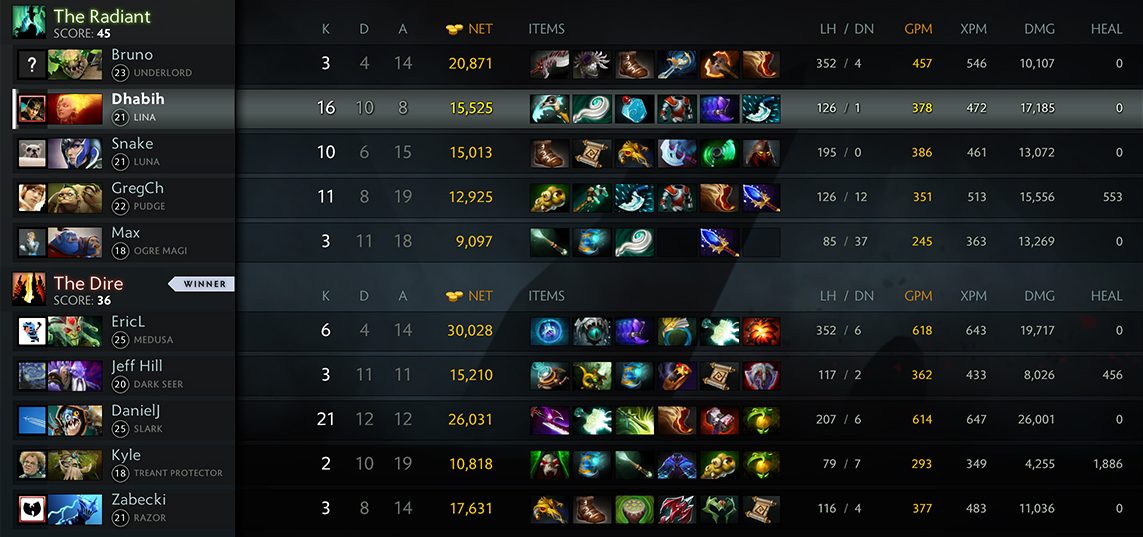
\includegraphics[scale=0.39]{results-summary}
\caption{An example of a match summary in the game `Dota 2'.}
\label{fig:results-summary}
\end{figure}
Values included in the match summary can be roughly separated into two types: class based and regression based.
For example in many games players have the ability to buy items.
These items are usually represented as numbers in match summary, but nearby values usually do not have much in common.
Therefore, if such variables have to be predicted, a classification method should be used is a good approach.

On the other hand something like players score is a value which increases progressively, therefore nearby values have similar significance.
In such cases regression techniques would work better.
\section{Requirement Analysis}
The projects aimed to produce a system that would be able to predict match summary data from players' history.
\begin{itemize}
\item The system must be able to work with data from different games, as long as it is formatted properly.
\item The predictions should be based on skills of all players in the match, not just the player for which predictions are being made.
\item The system should be able to maintain a belief state about a player skill through time and make time-sensitive predictions, not the same prediction for all matches.
\item The system should be able to make predictions in under a minute after being trained, on my machine\footnote{Specifications of machine's hardware are given in the project proposal}.
\item The mean squared error of system's predictions should be less than one half of player's variance for that variable.
\end{itemize}
\label{requirements-error}
\textbf{Regarding the last point}: in the project proposal my success criteria contained a mistake and had 'standard deviation' instead of 'variance', which made the success criteria almost impossible to achieve.
As it currently stands the systems deviation is squared, while original deviation is not, which means that achieving this requirement gets more difficult the larger the original deviation is.
This also makes a big difference once the variables are normalised, since squaring values less than one decreases it and makes achieving this result easier.
In my evaluation I will analyse the results as though the success criteria was stated as above.
\section{Starting Point}
\noindent
At the beginning of the project I had:
\begin{itemize}
\item Basic knowledge of artificial intelligence from \emph{Artificial Intelligence I} Part IB course.
\item Programming experience in Python (acquired by working on personal projects) and Java (acquired by completing courses in first two years of the tripos).
\item Knowledge of probability rules and Bayes' theorem from A-Level maths and math courses in the first two years.
\end{itemize}
During the course of the project I had to gain following qualities:
\begin{itemize}
\item Understanding of Bayes' inference and its use in ranking.
\item Understanding of various machine learning techniques.
\item Familiarity with the chosen ML library (Tensorflow).
\item Knowledge of \LaTeX\ and related packages (such as Tikz for graphs) to write-up this dissertation.
\end{itemize}
\section{Theoretical Background}
\subsection{Probability background}
There are a few probability rules, which are used in this model.
\paragraph{Sum rule}
Sum/Integral rule allows us to remove unneeded variables from our probability estimates:
\begin{equation*}
P(A) = \int\limits_{B}P(A,B) = \sum\limits_{B}P(A,B)
\end{equation*}
\paragraph{Product/Chain rule}
Product rule allows us to calculate joint probabilities only using conditional probabilities and priors:
\begin{equation*}
P(A,B) = P(A\mid B)P(B)
\end{equation*} 
\paragraph{Bayes' theorem}
I will be using Bayes' networks and inference in my system, which is based on Bayes' theorem:
\begin{equation*}
P(A\mid B) = \frac{P(B\mid A)P(A)}{P(B)}
\end{equation*}
\begin{itemize}
\item $\boldsymbol{P(A)}$ and $\boldsymbol{P(B)}$ are the probabilities of observing $A$ and $B$, called \emph{prior}s.
\item $\boldsymbol{P(A \mid B)}$ is the probability of observing $A$ given $B$, called \emph{posterior}.
\item $\boldsymbol{P(B \mid A)}$ is the probability of observing $B$ given $A$, called \emph{likelihood}.
\end{itemize}
\subsection{Machine Learning}
Machine learning allows computers to make predictions on data by learning from past examples and without being explicitly programmed.
The aim of my project was to create an algorithm which could work with any game, therefore machine learning was the perfect set of techniques to apply.

Since I decided to use machine learning in my project I had to get some background in the area.
Unfortunately, computer science course is in Lent term, which is too late, therefore I attended a similar course in Engineering department in Michaelmas term, before beginning the work on the theory.

After I have finished my research, I have decided to try the following machine learning techniques in my projeject:
\begin{itemize}
\item Naive bayes (NB)
\item Linear Regression (LinReg)
\item Logistic Regression (LogReg)
\item Polynomial Regression (PolReg)
\item Ridge Regression (RidReg)
\item Neural Networks (NN)
\item Support Vector Machines (SVM)
\item Gaussian Processes (GP)
\item Random Forests (RF)
\end{itemize}
\subsection{Over and under fitting}
When training an algorithm a decision has to be made when to stop the training, this is difficult decision and is usually made using some kind of heuristic.
If the training is stopped too early it leads to under-fitting, if it is stopped too late, it leads to over-fitting, in both cases the algorithm performs below optimum.
\paragraph{Under-fitting}
An under-fit algorithm cannot model the training data well and is not suitable.
It is often easy to detect using a good loss metric.
The basic solution is to use more complex model or train longer.
\paragraph{Over-fitting}
An over-fit algorithm models the training data too well, the algorithm learns the noise in the training data.
Noise is random, therefore it will be different in the real/test data.
By modelling the noise in the training data, the real world-performance is decreased.
Over-fitting is a bigger problem, since it is much more difficult to detect, therefore different methods are usually used to prevent it.
I outlined some of the methods I used in subsection \ref{overfitting}.
\section{Software Engineering Techniques}
\subsection{Workflow}
\begin{figure}[ht]
\centering
%\begin{tikzpicture}
%    \draw [domain=12.566:25.133,variable=\t,smooth,samples=300]
%        plot ({\t r}: {0.008*\t*\t});
%    \draw (-6,0) -- (6,0);
%    \draw (0,-6) -- (0,6);
%    \node[] at (6,6) {}; 
%\end{tikzpicture}
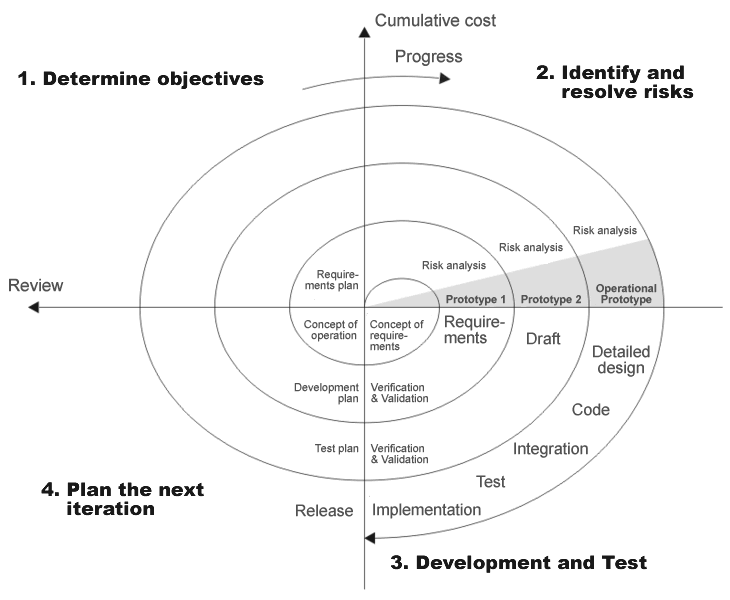
\includegraphics[scale=0.5]{spiral-model}
\caption{Agile approach using spiral model.}
\label{fig:spiral-model}
\end{figure}
I have decided to use an agile approach of working on this project, seen in figure \ref{fig:spiral-model}, since I was not sure exactly how the algorithm should work at the start of the project.
The project would be done in two phases:
\begin{enumerate}
\item Primary research would be done during the second half of Michaelmas term.
A prototype would be developed during the Christmas break.
\item At the beginning of Lent term the prototype would be evaluated.
In the first two weeks of February the theory would be improved using insights gained during the development of the prototype.
In the second two weeks of February the prototype would be refactored to comply with changes in the theory.
At the beginning of March the revised implementation would be evaluated.
\end{enumerate}
This approach allowed me to incorporate the knowledge I gained during the evaluation of a prototype into the final version of the algorithm.
\subsection{Version Control}
Git was used for version control.
Frequent commits were made after every self-contained change.
This allowed me to roll-back to a previous version of the project when a mistake was made.
It also allowed me to compare and evaluate different versions of a specific component.
The repository was hosted on GitHub\footnote{github.com} which allowed me to work on the project from multiple machines.
\subsection{Backup}
The code was continuously synchronised to Dropbox\footnote{dropbox.com}.
Weekly checkpoints were saved to an external hard drive.
\section{Tools used}
\subsection{Programming Language and ML Libraries}
Machine learning is one of the key elements of this project, therefore I needed a library that would implement key techniques used in ML for me, so that I don't have to write them myself.
I have compared a number of libraries (such as Tensorflow\footnote{tensorflow.org} and Torch\footnote{torch.ch}).
I was primarily interested in how much functionality they provide, their performance and how easy it would be to use them.

I have compared their functionality by completing standard machine learning task, such as creating a neural network to classify images in the MNIST\footnote{yann.lecun.com/exdb/mnist} dataset.
Performance was compared by timing how long it would take to achieve 99\% accuracy, in most cases it came down whether GPU acceleration was supported.
Since I would have to learn how to use the chosen library in detail, I also paid attention to the amount of support material available.
I took note of quality of documentation and also compared number of questions and answers on StackOverflow.

In the end I have arrived at the conclusion that they all provided required functionality and were similarly easy to use, but API for most of them were written in different languages.
I did not want to learn a new language in addition to learning a new library, therefore I decided to use TensorFlow, API for which was written in Python, a language I was most comfortable writing code in.
TensorFlow is a low-level library, in which each layer of neural network has to be constructed explicitly, I did not need that level of customisation, therefore I used Keras\footnote{keras.io} to help me build the neural networks.

Additionally Python has a higher level machine learning library called scikit-learn\footnote{scikit-learn.org}.
It provides easy way to quickly implement many machine learning methods, this library was used to evaluate prototype evaluation.
To a lesser extent Python was also chosen since it has a package manager\footnote{pypi.python.org/pypi/pip}, which makes it much easier to install additional packages.

\subsection{IDE}
Pycharm was chosen as the integrated development environment (IDE) for the project.
Pycharm has all of the core features of an IDE, such as syntax highlighting, autocompletion, code execution, etc.
The use of an IDE streamlined the process of development and allowed me to focus on improving the algorithm rather than worrying about language syntax or library functions signatures. 


\chapter{Implementation}
This chapter discusses design and implementation of the prediction system produced.
The system was made in two stages: first a prototype was made, tested and analysed.
Based on the result of the analysis a better system was designed and implemented.
The main system consists of two models: prediction model and skill update model.

Prediction model is used to make predictions based on the estimated skills of the players and to calculate player performance based on match results.
Skill update model is used to estimate the skills of the players at a particular time using past performances.
\section{Installation of required libraries}
Python has a package index (PyPI) which is used to distribute most available packages.
The PyPI provides a tool called \emph{pip} which can manage package/library installation, it can be installed on Ubuntu 16.04 using:
\begin{minted}[bgcolor=lightgray, texcl=true]{bash}
$ sudo apt install python3-pip
\end{minted}
After pip is installed all required packages can be installed using:
\begin{minted}[bgcolor=lightgray, texcl=true]{bash}
$ sudo pip install <package name>
\end{minted}
Pip will manage all of the required dependencies and put the package files in the correct directories.
\section{Data Collection and Pre-processing}
\subsection{Collecting the data}
To train and evaluate my algorithm I had to find a complex dataset which would have different types of variables for me to predict.
I decided to use a game called "Dota 2" for several reasons:
\begin{itemize}
\item Summary of each professional match is publicly available and easily accessible through the provided API.
\item "Dota 2" is one of the leading E-Sports with hundreds of professional matches each year, which provided me with plenty of data points.
\item The game requires a lot of skill with very little amount of luck involved, which makes it very suitable to prediction.
\item The game is team-based and requires a lot of co-operation, which makes it more difficult to predict using classical rating algorithms.
\end{itemize}
\begin{figure}

\end{figure}
\subsection{Pre-processing}
\paragraph{Cleaning the data}
The API which provides the summaries sometimes returns incomplete data with some of the values, such as the outcome of the match, missing.
I had to find and remove all data points which did not contain complete set of results.
\begin{figure}[ht]
\centering
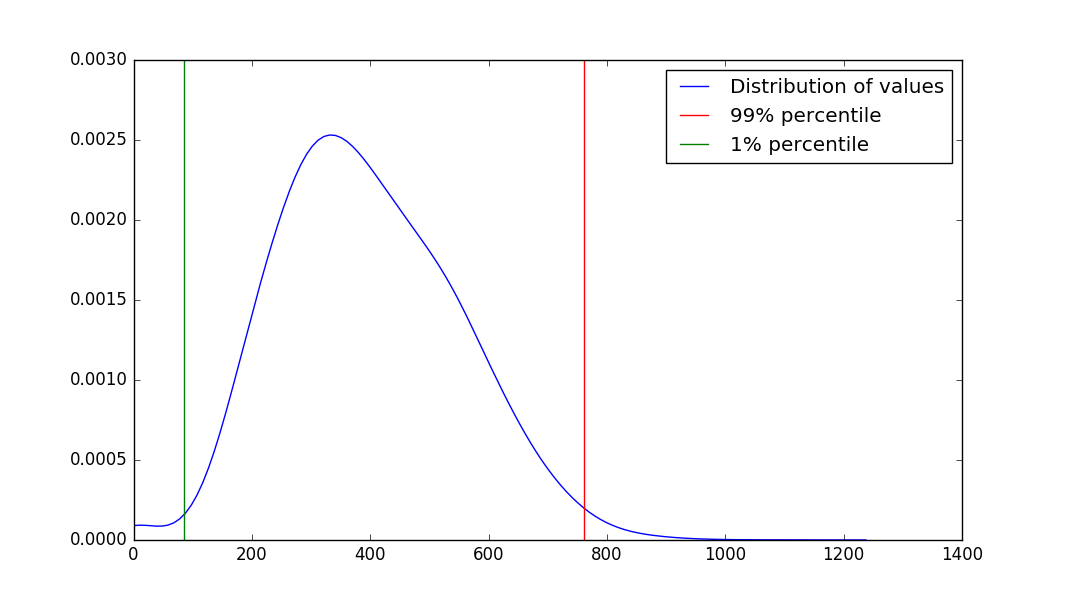
\includegraphics[scale=0.5]{outliers}
\caption{The distribution of values one of the variables.}
\label{fig:outliers}
\end{figure}
\paragraph{Outliers}
Most variables contain some outliers which are extreme cases.
In some cases the maximum value is almost twice as high as the 99\% percentile, as can be seen in figure \ref{fig:outliers}.
To simplify the learning for the algorithm I decided to clip all the value for each variable between the 1st and 99th percentile.
\paragraph{Standardisation}
Some of the variables in the summary occur over much bigger scales than others.
Most machine learning algorithms would not train properly and would prioritise predicting large variables more accurately than smaller ones.
I would like to consider all variables with equal priority, therefore I had to standardise the data.
To standardise data a simple transformation should be applied to all data points:
\begin{equation*}
x' = \frac{x - \mean{x}}{\sigma}
\end{equation*}
Where $\mean{x}$ is the mean of $X$ and $\sigma$ is its standard deviation
\paragraph{Normalisation}
During the analysis of data I decided that the data is better modelled using a gamma distribution.
Gamma distribution can only represent positive numbers, therefore I could not use standardisation for this dataset.
Instead I used normalisation which also rescales the values, but keeps them all positive, it uses the following transformation:
\begin{equation*}
x' = \frac{x - \min(X)}{\max(X)-\min(X)}
\end{equation*}
\section{First Prototype}
Frequently the main problem in machine learning is the generation of correct features to represent the data.
In my case I had summaries of more than twenty thousand matches.
Most players had a few hundred matches in the dataset.
Summary for each match is represented as a dictionary of key-value pairs (in JSON\footnote{json.org} format), overall there are more than 200 values per summary, an example of a summary can be found in Appendix \ref{statexample}.
This meant that using raw data for input would be impractical, therefore some kind of aggregation had to be created.

\subsection{Simple mean and variance}
At first I tried using means and standard deviations of players results as features.
While this approach made predictions which were better than just predicting variable mean, they weren't very good.
A variety of machine learning techniques were tried, including: Neural Networks (NN), Support Vector Machines (SVM), Gaussian Processes (GP), Ridge Regression (RR) and Naive Bayes (NB).
NN, SVM and NB were used for classification variables, while GP and RR were used for regression.
All of the methods had similar performance, which indicated that features generated were not sufficient.
To improve the features I first tried putting a limit on how many matches were used to calculate player's mean and average, while this improved performance a bit, it remained very low.
Next thing to try was rating players based on their performance in each variable.

\subsection{Rating of players}
The easiest algorithm I found for rating players was TrueSkill, since it offered rating games with multiple players and there was a library\footnote{trueskill.org} for python which provided the functionality.
TrueSkill only uses the final ranking of the individual at the end of the match, rather than absolute value, therefore some informations is lost.
This also meant that I had to do further processing on the data to convert raw values into rankings.
This was mostly straightforward, one thing to note is that some rankings (such as death count) had to be reversed, since players try to keep those results low rather than make them high.

Such ad-hoc use of TrueSkill meant that one of the assumptions behind the algorithm was not met:
the algorithm assumes that all players are competing against each other, but in reality they are separated in two teams.
This meant that resulting ratings were not very accurate.
Player skills were then used as features for machine learning techniques.
This approach generated much better results than simple mean and variance, with best variable achieving $R^2$ value of 0.43.
Although this is much better than previous results, it was below the required value of 0.5.

\subsection{Analysis of different machine learning techniques}
%TODO add figure here showing the results
As said above most of the techniques provided similar results.
In the end I decided to use neural networks as my main technique for the following reasons:
\begin{itemize}
\item Neural networks can do both regression and classification, thereby I will only have to focus on properly learning and understanding one technique.
\item One neural network can estimate values for multiple results, thereby reducing the complexity of the system and increasing efficiency.
\item Chosen library (Tensorflow) has better support for neural networks than other techniques.
\end{itemize}

\subsection{Analysis of the prototype}
\begin{figure}[ht]
\centering
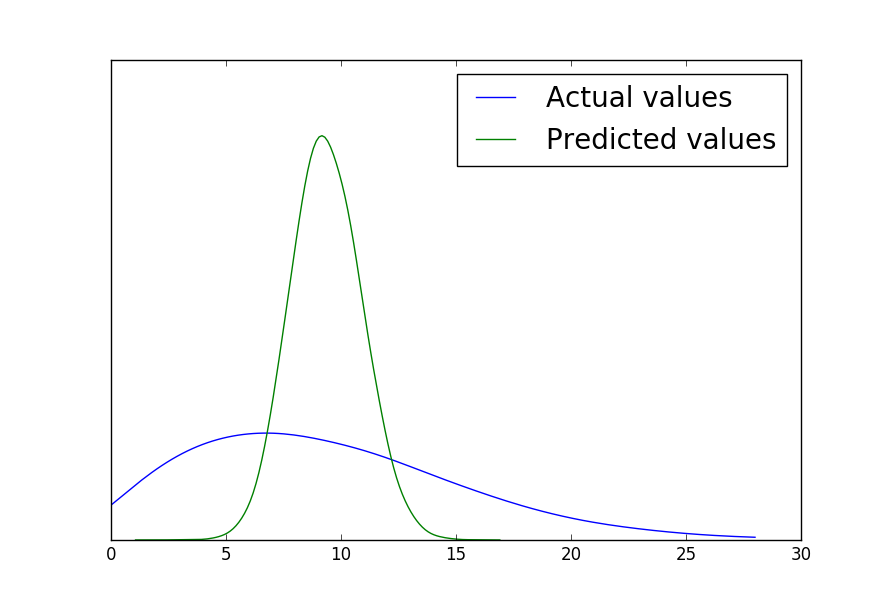
\includegraphics[scale=0.5]{predicted_assists}
\caption{Distribution of predicted values vs.\ actual variable distribution}
\label{fig:variablerange}
\end{figure}
During analysis of predictions produced by the prototype, I observed that the range of predictions was much smaller than the actual range for most variables.
An example of this can be seen on figure \ref{fig:variablerange}, where predictions roughly range from 5 to 15, while actual variable range is roughly 0 to 30.
In addition, most of the machine learning techniques had similar predictive performance.
These two facts combined led me to believe that the problem was with quality of features.

\subsection{Required refactoring and redesign}
To create better features I decided to modify the structure of the TrueSkill graphical model to remove the wrong assumptions.
This required adding dependency links between player ranks and their teams.
Additionally, I decided to use machine learning techniques throughout to calculate player ranks, rather than using hard-coded rules, since I do not know which variables are important.

I also decided to use a Bayesian approach because it reduces the risk of overfitting at the expense of increasing the risk of underfitting.
Since underfitting can be solved much easier, by increasing the size of the model for example, it made the training process much easier.
\section{Final System}
\subsection{Choosing distributions for different variables}
\begin{figure}[ht]
\centering
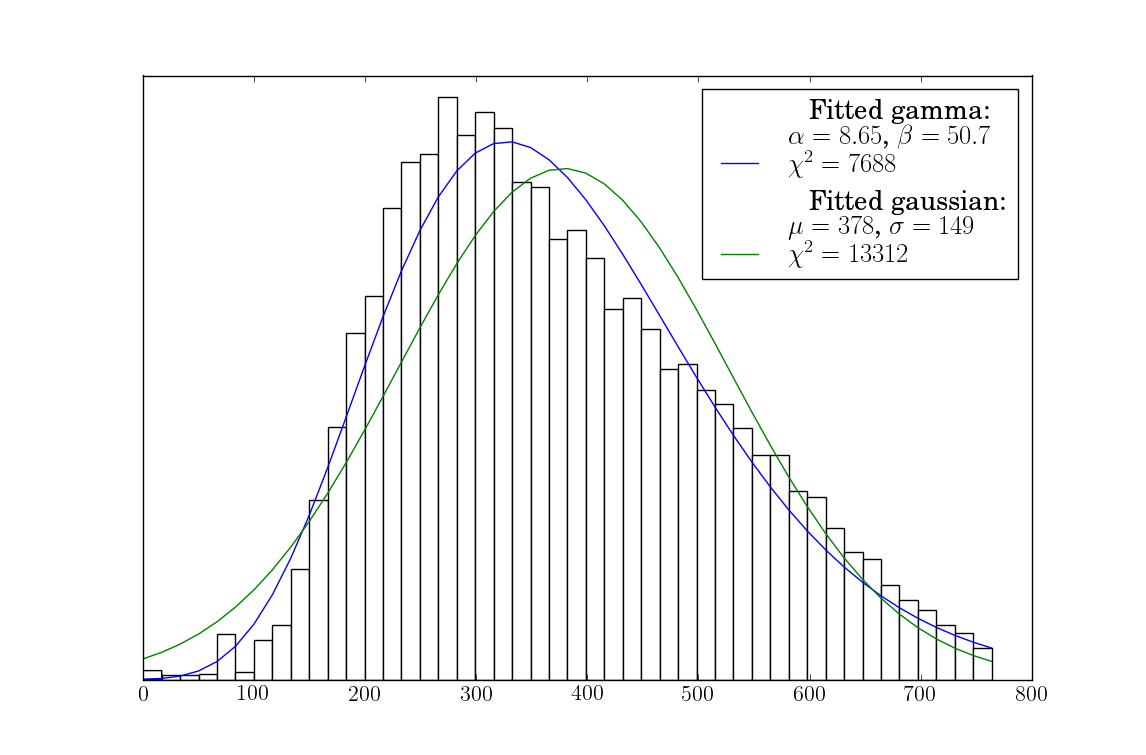
\includegraphics[scale=0.5]{fitted-distributions}
\caption{Fitted gaussian and gamma distributions on one of the variables.}
\note{Gamma distribution has a lower $\chi^2$ value, therefore it is a better fit.}
\label{fig:fitted-distributions}
\end{figure}
When predicting the values for each regression-based variable, rather than predicting the probability for each value independently, it is better to use a distribution to predict the probabilities for all values.
To decide which distribution fits each variable best, I used \emph{method of moments} to fit each potential distribution to all observed values of the variable.
Then I used \emph{goodness of fit} to decide which of the potential distributions is best.
\paragraph{Method of Moments}
To fit a distribution its parameters have to be estimated.
Parameters for most distributions can be easily expressed in terms of mean and variance of the data.
For example for Gamma distribution the equations are:
\begin{equation*}
k= \mu^2/\sigma^2
\qquad
\theta = \sigma^2/\mu
\end{equation*}
\paragraph{Goodness of fit}
To estimate how well the distribution fits the data use chi-squared test can be used, which measures the sum of differences between observed and expected outcome frequencies:
\begin{equation*}
\chi^2 = \sum_{i=1}^{n} \frac{(O_i - E_i)^2}{E_i}
\end{equation*}
Where $O_i$ is the observed frequency and $E_i$ is the expected frequency.
\subsection{Player skills}
Every game is different and trying to pick specific set of skills for each one, would not be practical.
Therefore, I decided to make an assumption that players skill in a game can be described by $n$ real numbers.
Such $n$ will be different for each game and therefore is a hyper parameter in my model.
Since the system can never be sure on the exact skill values for each player, skills of each player are represented as vector of Gaussian distributions with size $n$.
\subsection{Neural networks}
\begin{figure}[ht]
\centering
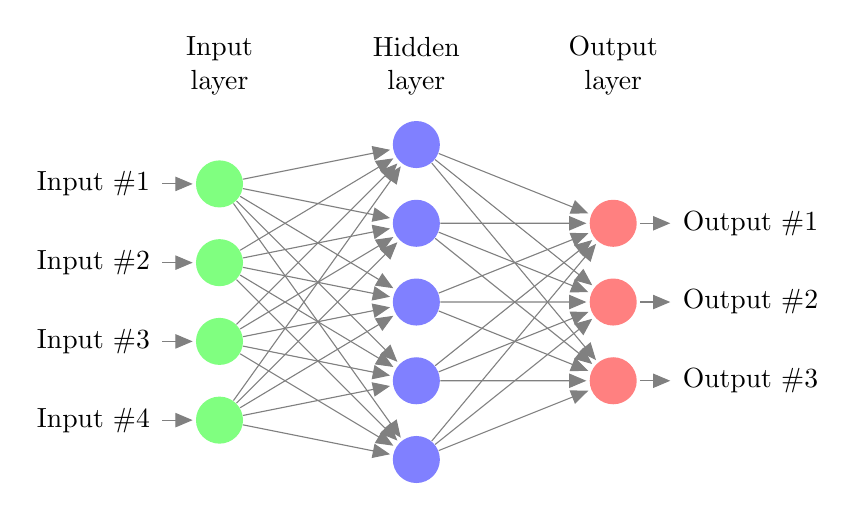
\begin{tikzpicture}[shorten >=1pt,->,draw=black!50, node distance=\layersep]
    \tikzstyle{every pin edge}=[<-,shorten <=1pt]
    \tikzstyle{neuron}=[circle,fill=black!25,minimum size=17pt,inner sep=0pt]
    \tikzstyle{input neuron}=[neuron, fill=green!50];
    \tikzstyle{output neuron}=[neuron, fill=red!50];
    \tikzstyle{hidden neuron}=[neuron, fill=blue!50];
    \tikzstyle{annot} = [text width=4em, text centered]

    % Draw the input layer nodes
    \foreach \name / \y in {1,...,4}
    % This is the same as writing \foreach \name / \y in {1/1,2/2,3/3,4/4}
        \node[input neuron, pin=left:Input \#\y] (I-\name) at (0,-\y) {};

    % Draw the hidden layer nodes
    \foreach \name / \y in {1,...,5}
        \path[yshift=0.5cm]
            node[hidden neuron] (H-\name) at (\layersep,-\y cm) {};
	
	% Draw the output layer nodes
	\foreach \name / \y in {1,...,3}
        \path[yshift=-0.5cm]
            node[output neuron,pin={[pin edge={->}]right:Output \#\y}] (O-\name) at (2*\layersep,-\y cm) {};	

    % Connect every node in the input layer with every node in the
    % hidden layer.
    \foreach \source in {1,...,4}
        \foreach \dest in {1,...,5}
            \path (I-\source) edge (H-\dest);

    % Connect every node in the hidden layer with the output layer
    \foreach \source in {1,...,5}
    		\foreach \dest in {1,...,3}
        		\path (H-\source) edge (O-\dest);

    % Annotate the layers
    \node[annot,above of=H-1, node distance=1cm] (hl) {Hidden layer};
    \node[annot,left of=hl] {Input layer};
    \node[annot,right of=hl] {Output layer};
\end{tikzpicture}
\caption{An example of fully connected feedforward neural network with one hidden layer.}
\label{fig:neural-network}
\end{figure}
I decided to use neural networks in my system, therefore I had to learn basic theory behind them and how to construct them.
Neural networks are usually made up of three types of layers: input, hidden and output.
The size of the input and output layer are determined by the data being processed, deciding on the size of hidden layers is more difficult.
If the hidden layers are too small under-fitting can occur, similarly if the hidden layers are too big or there too many of them over-fitting can occur.
\paragraph{Perceptron}
Each layer of a NN is composed of a number of perceptrons.
Perceptron is a simple linear classifier which is can be described by the following equation:
\begin{equation*}
y = \sigma(\bs{w\cdot x}+b)
\end{equation*}
Where $y$ is the output, $\sigma()$ is the activation function, $\bs{w}$ a vector of weights, $\bs{x}$ is a vector of inputs and $b$ is the bias.

\paragraph{Types of activation function}
There are several types of activation function that can be used in neural networks, I considered the following:
\begin{description}[labelwidth=\widthof{\bfseries Rectified Linear Unit (ReLU) }]
\item[Identity] $\sigma(x) = x$
\item[Rectified Linear Unit (ReLU)] $\sigma(x) = \max(x,0)$
\item[Softplus] $\sigma(x) = \ln(1+e^x)$
\item[TanH] $\sigma(x) = \tanh(x)$
\end{description}
Most of them map the value of $x$ onto a specific range, which is useful if the output must also fall in a certain range.
Normally the activation function is based on which layer the perceptron is in.
Activation functions such as ReLU are also useful in hidden layers to produce a non-linear transformation.

\paragraph{Type of NN}
There are many types of neural networks, I decided to use the simplest one: \emph{fully connected}, \emph{feedforward} neural network.
\begin{description}[labelwidth=\widthof{\bfseries Fully connected }]
\item[Fully connected] Input for a perceptron in layer $n$ is composed of output of each perceptron in layer $n-1$.
\item[Feedforward] The data only flows one way in the network, there are no loops.
\end{description}
An example of a structure of such neural network can be seen in figure \ref{fig:neural-network}.

\subsection{System overview}
\begin{figure}[ht]
\centering
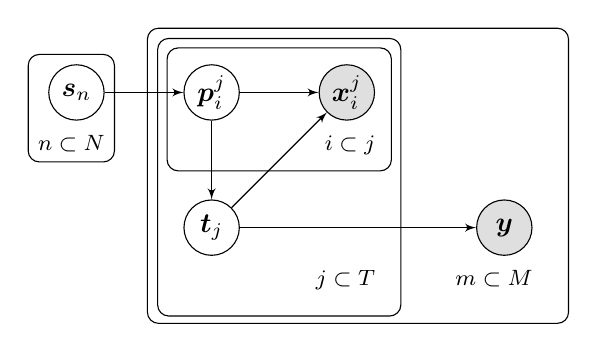
\begin{tikzpicture}
\tikzset{edge/.style = {->,> = latex'}}
\node[latent] (p) [] {$\bs{p}_i^j$};

\node[latent] (t) [below=of p] {$\bs{t}_j$};
\draw[edge] (p) to (t);

\node[obs] (x) [right=of p] {$\bs{x}_i^j$};
\draw[edge] (p) to (x);
\draw[edge] (t) to (x);

\node[obs] (y) [right=3cm of t] {$\bs{y}$};
\draw[edge] (t) to (y);

\plate[inner sep=0.2cm] {i} {(p)(x)} {$i\subset j$};
\plate[inner sep=0.32cm] {j} {(p)(x)(t)} {$j\subset T$};
\plate[inner sep=0.45cm] {m} {(p)(x)(t)(y)} {$m\subset M$};

\node[latent] (s) [left=of p] {$\bs{s}_n$};
\draw[edge] (s) to (p);
\plate {n} {(s)} {$n\subset N$};
\end{tikzpicture}
\caption{Summed up view of the prediction model.}
\note{There are $N$ players tracked by the system, participating in $M$ matches.
In each match there are $T$ teams.
$\bs{x}_i^j$ are the results of player $i$ in team $j$ and $\bs{y}$ are the overall match results.
All variables are vectors.}
\label{fig:model-simple}
\end{figure}

The model assumes that there are two types of results for each match:
\begin{itemize}
\item Player specific results, such as the amount of gold earned or the number of enemies killed.
\item Overall match results, such as which team won or how long the match took.
\end{itemize}
The naive approach is to have only one neural network which takes player skill estimates as inputs and outputs predictions of results.
There are several problems with such system:
\begin{itemize}
\item As the size of input grows, so does the size of the neural network required to accurately process them.
This leads to massive neural network which takes a long time to process data and therefore quite inefficient.
\item As the size of the neural network grows, the number of examples required to train it also increases.
Although I had quite a large data-set I judged that it was not large enough to properly train such a big network.
\end{itemize}
Therefore I made a few assumptions to create a graphical model which resolves those problems.
The assumptions are:
\begin{itemize}
\item Skills of all players playing on the same team can be combined into a smaller set of skills.
\item Player specific results only depend on the skills of relevant player and combined skills of each team taking part in the match.
\item Overall match results only depend on combined team skills.
\end{itemize}
The summary of resulting system is seen in figure \ref{fig:model-simple}.

There are two models in the system: predicting results from inferred player skills and inferring player skills from their match history.
An example of a prediction model made for a game in which four players play in two teams can be seen in figure \ref{fig:four-player-model} and a factor graph expansion can be found in Appendix \ref{factor-graph}.
The skill update model is the same for all games and can be seen in figure \ref{fig:skill-update}.

Training both the variable prediction model and skill update model at the same time would greatly increase the data required for processing.
It will also raise some difficult problem such as \emph{vanishing gradient}.
Unfortunately I did not have enough time to solve these problems properly.
Instead, I decided to use the technique called \emph{coordinate descent}, to optimise the models alternatively.
\paragraph{Coordinate descent}
When there are multiple parameters to optimise, instead of optimising them at the same time they can be optimise alternatively.
Each parameter is optimised until it reached a stable value, then the next parameter is optimised.
Once each parameter is optimised, loop back and start again from the first one.
This cycle is repeated until all parameters reach sufficiently stable values across multiple cycles.

\subsection{Prediction model}
\begin{figure}[ht]
\centering
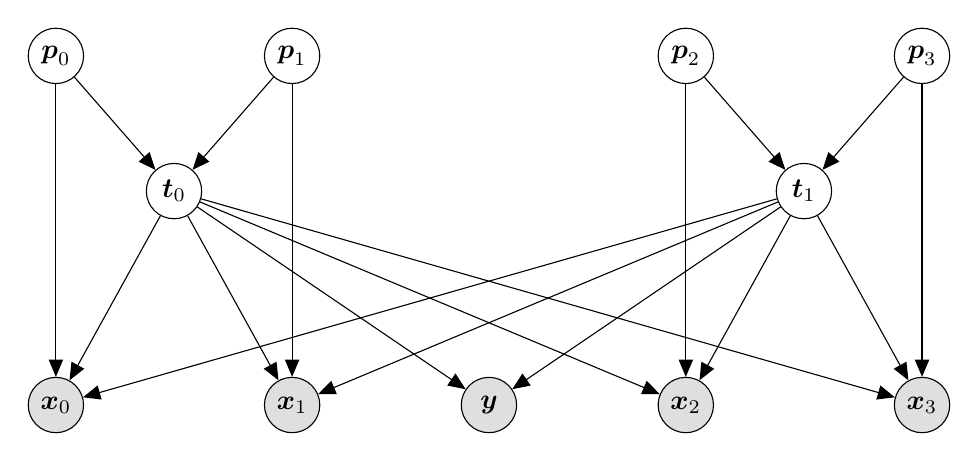
\begin{tikzpicture}
	% Team results
	\node[obs] (y) [] {$\bs{y}$};	
	
	% Team performances
	\node[latent] (t0)[above=2cm of y, xshift=-4cm] {$\boldsymbol{t}_0$};
	\node[latent] (t1)[above=2cm of y, xshift=4cm] {$\boldsymbol{t}_1$};
	
	% Player results
 	\node[obs] (x0)[below= 2cm of t0, xshift=-1.5cm] {$\boldsymbol{x}_0$};
 	\node[obs] (x1)[below= 2cm of t0, xshift=1.5cm] {$\boldsymbol{x}_1$};
 	\node[obs] (x2)[below= 2cm of t1, xshift=-1.5cm] {$\boldsymbol{x}_2$};
 	\node[obs] (x3)[below= 2cm of t1, xshift=1.5cm] {$\boldsymbol{x}_3$};
 	
 	% Player performances
 	\node[latent] (p0)[above=of t0, xshift=-1.5cm] {$\boldsymbol{p}_0$};
 	\node[latent] (p1)[above=of t0, xshift=1.5cm] {$\boldsymbol{p}_1$};
 	\node[latent] (p2)[above=of t1, xshift=-1.5cm] {$\boldsymbol{p}_2$};
 	\node[latent] (p3)[above=of t1, xshift=1.5cm] {$\boldsymbol{p}_3$};
 	
 	%Player to team performance
 	\edge[] {p0,p1} {t0};
 	\edge[] {p2,p3} {t1};
 	
 	%Player results
 	\edge[] {p0,t0,t1} {x0};
 	\edge[] {p1,t0,t1} {x1};
 	\edge[] {p2,t1,t0} {x2};
 	\edge[] {p3,t1,t0} {x3};
 	
 	%Team performance
 	\edge[] {t0,t1} {y};
 	
	
\end{tikzpicture}
\caption{An example of an inference model for four players in two teams.}
\note{Grey circles represent observed values and white circles represent latent variables.}
\label{fig:four-player-model}
\end{figure}
There are four variables in this model: $\bs{x},\bs{y},\bs{t},\bs{p}$.
To make predictions we would like to calculate $P(\bs{x},\bs{p})$ and $P(\bs{y},\bs{p})$.
As was said above, calculating these probabilities directly is expensive, by expressing them using the terms in the model, redundant links can be removed greatly simplifying the computation.
First the conditionals probabilities are expressed according to model structure:
\begin{equation*}
P(\bs{x}_i,\bs{t},\bs{p})\quad \text{and} \quad P(\bs{y},\bs{t},\bs{p})
\end{equation*}
Using product rule the joint probabilities are expanded into several conditional probabilities:
\begin{equation*}
P(\bs{x}_i,\bs{t},\bs{p}) = P(\bs{x}_i\mid\bs{t},\bs{p})P(\bs{t}\mid\bs{p})P(\bs{p})
\end{equation*}
Using the assumption that player results only depend on the skills of that player and team skills, most of the players can be integrated out, leaving:
\begin{equation*}
P(\bs{x}_i\mid\bs{t},\bs{p}) = P(\bs{x}_i\mid\bs{t},\bs{p}_i)
\end{equation*}
Doing the same to other parts leaves:
\begin{equation}
P(\bs{x}_i,\bs{t},\bs{p}) = P(\bs{x}_i\mid\bs{t},\bs{p}_i)P(\bs{t}\mid\bs{p})P(\bs{p})\qquad
P(\bs{y},\bs{t},\bs{p}) = P(\bs{y}\mid\bs{t})P(\bs{t}\mid\bs{p})P(\bs{p})
\label{eq:split-conditionals}
\end{equation}
Which is now expressed in terms of conditional probabilities we can calculate and priors which we know.

The skills of each player represent the prior on their performances.
Each player starts with their skill represented by $n$ standard Gaussians.
After each match, the parameters of those Gaussians are adjusted, such that for the next match the priors are different.

\paragraph{Neural Networks}
Conditional probabilities such as $P(\bs{x}_i\mid\bs{t},\bs{p}_i)$ are specific to every game and are most likely very complex.
In such cases I use machine learning techniques to approximate there probabilities, since this is a probability of a vector given other vectors, neural networks are the perfect candidate to use.
All of the variables in the model are defined using distributions, therefore neural networks must output the parameters of required distribution.
For example, for gamma distribution:
\begin{equation*}
P(\bs{x}_i \mid\bs{t},\bs{p}_i)=\text{gamma}(\bs{x}_i;\bs{k_\gamma}(\bs{t},\bs{p}_i), \bs{\theta_\gamma}(\bs{t},\bs{p}_i))
\end{equation*}
Where parameters $\bs{k_\gamma}$ and $\bs{\theta_\gamma}$ are outputs of a neural network with inputs $\bs{p}$ and $\bs{t}$ parametrised by $\bs{\gamma}$.

\subsection{Inferring player performance}
Player performance is a latent variable, therefore there are no values available to train a neural network.
To infer the performance of each player from the match results, the conditional probability $P(\bs{p}\mid\bs{t},\bs{x})$ has to be calculated.
Using Bayes' theorem this can be transformed to use conditional probabilities already known:
\begin{equation*}
P(\bs{p}\mid\bs{t},\bs{x}) = \frac{P(\bs{x}\mid\bs{t},\bs{p})P(\bs{t}\mid\bs{p})P(\bs{p})}{P(\bs{t},\bs{x})}
\end{equation*}
Unfortunately, because the conditional probabilities are calculated using neural networks, calculating the joint probability $P(\bs{t},\bs{x})$ is almost impossible.
Normal approach would be to use sum rule on the whole probability $P(\bs{p},\bs{t},\bs{x})$ and integrate $\bs{p}$ out:
\begin{equation}
P(\bs{t},\bs{x})=\int\limits_{\bs{p}\subset P} P(\bs{p},\bs{t},\bs{x}) d\bs{p}
\label{eq:performance-integral}
\end{equation}
That would require to do a sum over all possible weights in all of the neural networks, which is intractable. 

\paragraph{Variational Methods}
Using variational inference, the conditional probability $P(\bs{p}\mid\bs{t},\bs{x})$ can be approximated with a tractable distribution $q_{\bs{\theta}}(\bs{p}\mid\bs{t},\bs{x})$ with free parameters $\bs{\theta}$ that are close in KL-divergence to the exact posterior.
Therefore the KL-divergence has to be optimised, which is equivalent to maximising the evidence lower bound of the objective function (ELBO):
\begin{equation*}
\mathbb{E}_{q(\bs{p}\mid\bs{t},\bs{x})}\left[\frac{P(\bs{p},\bs{t},\bs{x})}{q_{\bs{\theta}}(\bs{p}\mid\bs{t},\bs{x})}\right]
\end{equation*}
Maximising the ELBO is a better than minimizing the evidence upper bound (EUBO), because the estimate always underfits the objective function, but EUBO can overfit which can decrease accuracy a lot.
If $q_{\bs{\theta}}(\bs{p}\mid\bs{t},\bs{x})$ is constructed such that it can be sampled from using Monte Carlo, then the integral from equation \ref{eq:performance-integral} can be approximated by a sum:
\begin{equation*}
\int\limits_{\bs{p}\subset P} P(\bs{p},\bs{t},\bs{x}) d\bs{p} \approx \frac{1}{k}\sum\limits_{k=1}^{K}\frac{P(\bs{p}^k,\bs{t},\bs{x})}{q_{\bs{\theta}}(\bs{p}^k\mid\bs{t},\bs{x})} \qquad k=1,\dots,K
\end{equation*}
where $\bs{p}^k$ is the $k$-th sample.

Team skills are also latent variables which have to be estimated from match results.
Another q-function has to be trained to estimate $P(\bs{t}\mid\bs{x},\bs{y})$.
%The complete graph of player performance inference model is shown in figure \ref{fig:q-model}.
%\begin{figure}[ht]
%\centering
%\begin{tikzpicture}
%	% Team results
%	\node[obs] (y) [] {$\bs{y}$};	
%	
%	% Team performances
%	\node[latent] (t0)[above=2cm of y, xshift=-4cm] {$\boldsymbol{t}_0$};
%	\node[latent] (t1)[above=2cm of y, xshift=4cm] {$\boldsymbol{t}_1$};
%	
%	% Player results
% 	\node[obs] (x0)[below= 2cm of t0, xshift=-1.5cm] {$\boldsymbol{x}_0$};
% 	\node[obs] (x1)[below= 2cm of t0, xshift=1.5cm] {$\boldsymbol{x}_1$};
% 	\node[obs] (x2)[below= 2cm of t1, xshift=-1.5cm] {$\boldsymbol{x}_2$};
% 	\node[obs] (x3)[below= 2cm of t1, xshift=1.5cm] {$\boldsymbol{x}_3$};
% 	
% 	% Player performances
% 	\node[latent] (p0)[above=of t0, xshift=-1.5cm] {$\boldsymbol{p}_0$};
% 	\node[latent] (p1)[above=of t0, xshift=1.5cm] {$\boldsymbol{p}_1$};
% 	\node[latent] (p2)[above=of t1, xshift=-1.5cm] {$\boldsymbol{p}_2$};
% 	\node[latent] (p3)[above=of t1, xshift=1.5cm] {$\boldsymbol{p}_3$};
% 	
% 	%Player to team performance
% 	\edge[] {t0} {p0,p1};
% 	\edge[] {t1} {p2,p3};
% 	
% 	%Player results
% 	\edge[] {x0} {p0,t0,t1};
% 	\edge[] {x1} {p1,t0,t1};
% 	\edge[] {x2} {p2,t1,t0};
% 	\edge[] {x3} {p3,t1,t0};
% 	
% 	%Team performance
% 	\edge[] {y} {t0,t1};
% 	
%	
%\end{tikzpicture}
%\caption{An example of an player performance inference graph.}
%\label{fig:q-model}
%\end{figure}


\subsection{Skill update model}
\begin{figure}[ht]
\centering
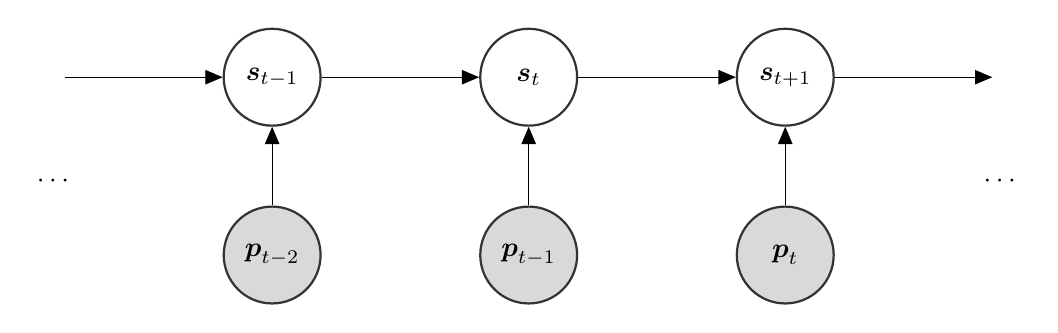
\begin{tikzpicture}
\tikzstyle{main}=[circle, thick, draw=black!80, minimum size=35pt, inner sep=2pt]
	%Skill chain
	\node[] (sn3) [] {};
	\node[main] (sn0) [right=2cm of sn3] {$\bs{s}_{t-1}$};
	\node[main] (sn)  [right=2cm of sn0] {$\bs{s}_t$};
	\node[main] (sn1) [right=2cm of sn] {$\bs{s}_{t+1}$};	
	\node[] (sn2) [right=2cm of sn1] {};	

	%Dots
	\node[] (d0) [below=of sn3] {$\cdots$};
	\node[] (d1) [below=of sn2] {$\cdots$};
	
	%Performance chain
	\node[main, fill=black!15] (p0) [below=of sn0] {$\bs{p}_{t-2}$};
	\node[main, fill=black!15] (p) [below=of sn] {$\bs{p}_{t-1}$};
	\node[main, fill=black!15] (p1) [below=of sn1] {$\bs{p}_{t}$};
	
	%Skill to skill
	\edge[] {sn3} {sn0};
	\edge[] {sn0} {sn};
	\edge[] {sn} {sn1};
	\edge[] {sn1} {sn2};	
		
	%Perormance to skill
	\edge[] {p0} {sn0};
	\edge[] {p} {sn};
	\edge[] {p1} {sn1};
\end{tikzpicture}
\caption{Skill update model}
\label{fig:skill-update}
\end{figure}
After every match the system updates its belief about the player's skills using the previous belief and player's performance in the match.
This forms a chain of beliefs about player's skill at each particular moment in time.
After each match, for each player the model updates the player skill using:
\begin{equation*}
P(\bs{s}_t) = P(\bs{s}_t\mid \bs{s}_{t-1},\bs{p}_{t-1}) = \mathcal{N}(\bs{s}_t;\bs{\mu_\lambda}(\bs{s}_{t-1},\bs{p}_{t-1}),\bs{\sigma_\lambda}(\bs{s}_{t-1},\bs{p}_{t-1}))
\end{equation*}
Where $\bs{\mu_\lambda}$ and $\bs{\sigma_\lambda}$ are outputs of the neural network\footnote{Code for this neural network is in Appendix \ref{code-example}.} with inputs $\bs{s}_{t-1}$ and $\bs{p}_{t-1}$, which is parametrised by $\bs{\lambda}$.

\subsection{Training neural networks}
To train the system the likelihood of the conditional probabilities has to be maximised and KL-divergence of all approximated functions has to be minimised.
To train a neural network a loss function is required.
\paragraph{Loss function for conditional probabilities}
All of the outputs of conditional probabilities are probability distributions, therefore we can use the probability density function (pdf) of the chosen distribution as the loss function.
The higher the pdf, the better the estimate, but loss function is minimised, therefore we need to negate the pdf to define loss.
For example a loss function for a Gaussian distribution would be:
\begin{equation}
\mathcal{L}(x,\mu,\sigma) = -\frac{1}{\sqrt{2\sigma^2\pi}}e^{-\frac{(x-\mu)^2}{2\sigma^2}}
\label{eq:gaussian-loss}
\end{equation}
where $x$ is the desired value and $\mu$ \& $\sigma$ are estimated parameters.

\paragraph{Optimising loss function}
The loss function is defined across the whole system, therefore we need to multiply the pdfs of all the distributions.
Multiplication is problematic due to two problems:
\begin{itemize}
\item It is computationally expensive
\item Multiplying small probabilities can lead to underflow, which will mean that the final probability might be equal to zero.
\end{itemize}
The log of the loss function is taken, it turns products into sums thereby reducing required computation and reduces the range of exponent preventing overflow and underflow:
\begin{equation*}
\mathcal{L} = \log\left(\prod_{p\subset P}p(x)\right) = \sum_{p\subset P}\log(p(x))
\end{equation*}
Since all probabilities are positive log of them is always defined, log is also a monotonically increasing function which means that decreasing log also decreases the function.

Taking log of the samples produced by the variational methods also reduces the variance of samples, which greatly decreases the number of samples required for approximation.
In my case I found that variance of samples is small enough that only one sample was required during training.

Computing the pdf itself also poses a problem, since potentially very small and very large values are multiplied together the pdf itself can underflow or overflow.
To prevent those problems, the log in the loss function can be pushed further in, e.g. Gaussian from equation \ref{eq:gaussian-loss} becomes:
\begin{equation*}
\mathcal{L}(x,\mu,\sigma) = \frac{\log(2)+\log(\pi)}{2}+\log(\sigma)+\frac{(x-\mu)^2}{2\sigma^2}
\end{equation*}
The optimising function can only change the parameters produced by the neural networks, therefore constants in the loss function do not matter and can be removed, leaving:
\begin{equation}
\mathcal{L}(x,\mu,\sigma) = \log(\sigma)+\frac{(x-\mu)^2}{2\sigma^2}
\label{eq:gaussian-log-loss}
\end{equation}

\paragraph{Minimising KL-divergence}
Recent paper on variational inference optimisation \cite{variationalmethods} mentions three methods of minimising KL-divergence:
\begin{description}[labelwidth=\widthof{\bfseries Entropy form }]
\item[FMC form] $\mathcal{L}(\theta) = \mathbb{E}_{q}[\ln P(\bs{x},\bs{p}) - \ln q_\theta(\bs{p}\mid\bs{x})]$
\item[Entropy form] $\mathcal{L}(\theta) = \mathbb{E}_{q}[\ln P(\bs{x}\mid\bs{p})] + \mathbb{H}[q_\theta]$
\item[KL form] $\mathcal{L}(\theta) = \mathbb{E}_{q}[\ln P(\bs{x}\mid\bs{p})] - \text{KL}(q_\theta \parallel P(\bs{p}))$
\end{description}
Through trial and error, I found that \emph{entropy} form worked best on my dataset.
Therefore final equation to be optimised for prediction model was:
\begin{equation*}
\mathbb{E}_{q\sim\bs{z}}[\ln P(\bs{x}_i\mid\bs{t},\bs{p}_i)+\ln P(\bs{y}\mid\bs{t})+\ln P(\bs{t}\mid\bs{p})+\ln P(\bs{p})] + \mathbb{H}[q_\theta(\bs{t}\mid\bs{x},\bs{y})] + \mathbb{H}[q_\psi(\bs{p}_i\mid\bs{x}_i,\bs{t})]
\end{equation*}
This way, all neural networks are optimised at the same time.
The loss equation for skill update model can be constructed similarly.
\paragraph{Restricting the range of the output}
Some of the parameters have to fall within certain range, but the neural output produced by a node in a neural network is usually not bound to any range.
This can be solved by using an appropriate activation function on the final layer of the neural network.
\emph{ReLU} is an obvious choice for enforcing positive values, but it is problematic in that the optimisation function may not properly adjust the weights of the NN.
Instead, I decided to use \emph{SoftPlus} activation function.

Although, sometimes different outputs of the same neural network must have different bounds placed on them.
Since the activation function is usually defined on the whole layer, it is frequently better to keep activation function of the last layer as \emph{linear} and apply appropriate activation function on each element individually.

\subsection{Prediction}
To predict the values for a particular match-up the players' skills corresponding to players in the match-up are taken and feed them into the top of the model.
Since the system tracks the skill of the players through time, the skill of players at the appropriate time has to be found.

\subsection{Restricting the time frame of training data}
\begin{figure}[ht]
\centering
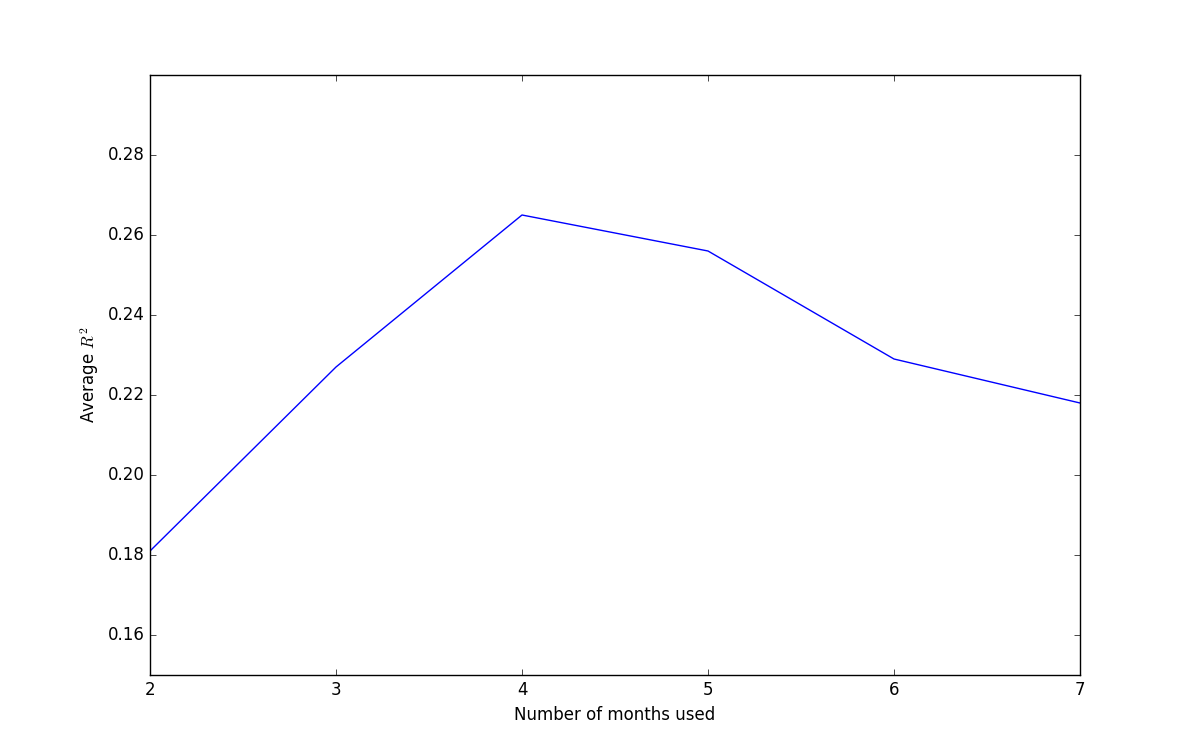
\includegraphics[scale=0.5]{time-variance}
\caption{Average $R^2$ with respect to time range of data considered.}
\note{Here it can seen that best choice would be around four months.
This correlates with the fact that the rules of the game change roughly seasonally.}
\label{fig:time-variance}
\end{figure}
Many popular multiplayer computer games change their rules a few times a year to keep the game fresh and players interested as well as to balance the game.
In addition, the strategies players employ evolve through time and different skills become more or less important in the game.
If the system is trained on the whole history of matches, it is optimised to predict results across the whole time-frame, but most of the time only predicting future events makes sense.
Therefore, to improve the accuracy of the system only the most recent matches are used for training, in which players employ current strategies.
Although, there is a trade-off: the smaller the time-frame the fewer matches are available for analysis.

\section{Summary}
In this chapter the structure and design of the main system was introduced and explained.
To design the main system, a graphical model was constructed, then conditional probabilities were estimated using neural networks.
Using neural networks for conditional probabilities, meant that Bayes' theorem could not be used to make a model for performance estimate.
To solve that problem variational methods were used to approximate the reverse conditional probability using sampling.

\chapter{Evaluation}
This chapter discusses how the final system was optimised and evaluated.
It introduces \emph{train/validation/test} split and how it is used to evaluate machine learning models.
In this chapter I also discuss how validation results can be used to optimise the model using \emph{hyper-parameter search}.

\section{Preprocessing}
Once neural networks have been trained, matches have to be processed in chronological order to update the player skills.
To make evaluation quicker a dictionary can be created which contains match id as keys and skills of the players taking part in that match.
Player skills have to be calculated before processing the match and updating them, to accurately reflect real world scenario.
\section{Train/Validation/Test split}
One of the most important rules when evaluating machine learning systems is that the algorithm must be tested on previously unseen data.
Therefore, right at the start the data can be split into two parts: \emph{train/validation} and \emph{test}.
\emph{Train/validation} set will be used to train the algorithm and adjust hyper-parameters.
\emph{Test} set will be used for evaluation of the algorithm.

\subsection{Preventing Over-fitting}

\label{overfitting}
Deciding on the length of training period is a difficult tasks.
If the training period is not long enough the algorithm will be under-fit.
Similarly, if the training period is too long, the algorithm might over-fit, as can be seen on figure \ref{fig:overfitting}.
Even if measures are taken to prevent over-fitting time will still be wasted.
There are several methods to prevent over-fitting:
\begin{description}
\item[Using simple models]
If the model has the correct complexity, it will only be able to learn the data and not the noise.
Another benefit of this approach is that training and prediction times are shorter.
Using this method the model can be trained until loss stops decreasing.
Unfortunately, if the model is too simple the model can suffer from under-fitting.

\item[Model regularization]
Another approach is to penalise complexity in the model.
For example the size of weights in neural networks can be limited to a certain value.
Unfortunately, this can also lead to under-fitting.

\item[Early stopping] 
Over-fitting can also be prevented by emulating testing scenario during training.
For that purpose the train/validation part is split into train and validation.
The algorithm is trained on train part and after every iteration it is tested on validation part.
When the validation error stops decreasing the training is stopped.
\end{description}
I decided to use validation since it does not suffer from potential of under-fitting and also has added benefit of allowing selection of hyper-parameters.
The best hyper-parameter combination can be found by first training the system using each combination and validating it, and then comparing the results of each validation.

\begin{figure}[ht]
\centering
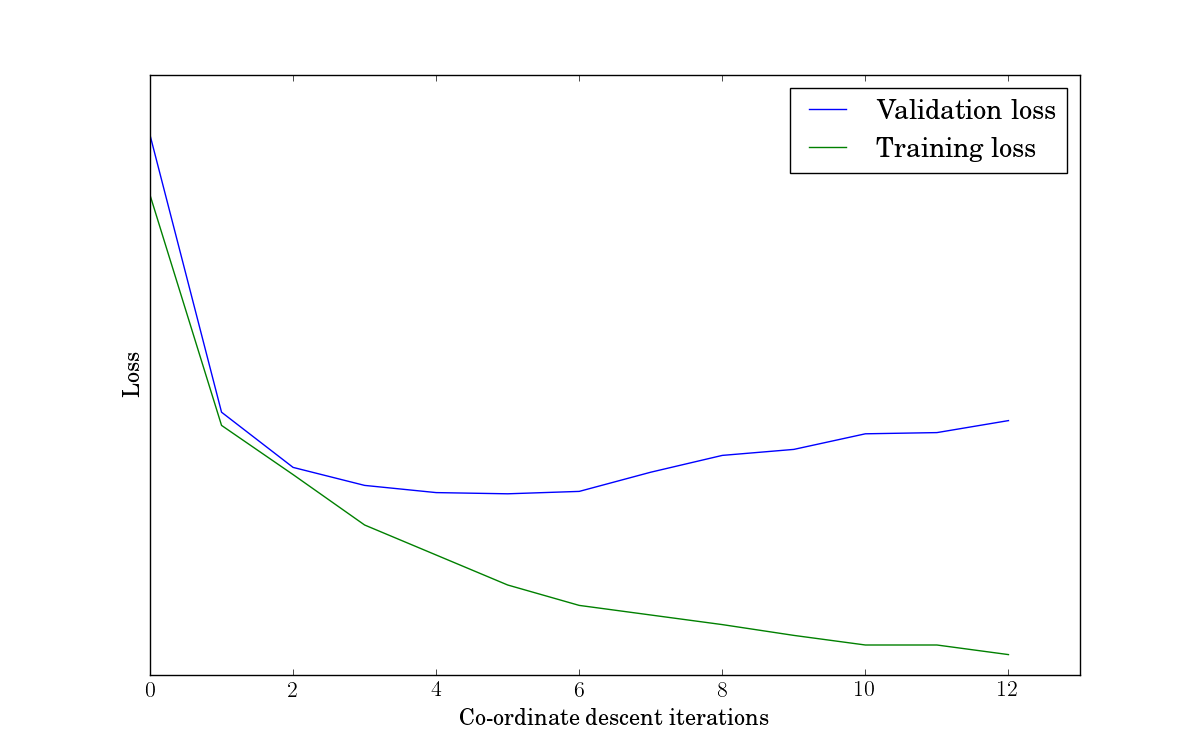
\includegraphics[scale=0.5]{overfitting}
\caption{Overfitting example.}
\note{In this case the optimisation should be stopped at the fifth iteration, after which training loss keeps decreasing, but validation loss starts increasing.}
\label{fig:overfitting}
\end{figure}

\subsection{Cross-validation}
If only one part of training data is used for validation, it might not properly represent the performance of the algorithm.
To combat that, cross-validation can be used: train/validation cycle is run multiple times, each time a new set is used for validation.
To ensure complete coverage of the train-set \emph{k-fold cross-validation} can be used: 
\begin{enumerate}
\item The train/validation set is divided into $k$ subsets.
\item A subset is picked that has not been validated on, the rest are used for training and it is used for validation.
\item Step two is repeated until all $k$ subsets have been validated on.
\item The results are averaged.
\end{enumerate}

\subsection{Split ratio}
When splitting the dataset into train/validation and test parts it is important to keep in mind the total size of the dataset.
Making the size of the test part too small can lead to statistically insignificant results and also increase the chance of sampling error.
On the other hand, making the size of training data too small can lead to under-fitting for the model.
I decided to use standard 80:20 train/test split using the Pareto principle.

\section{Hyper-parameter selection}
\begin{figure}[ht]
\centering
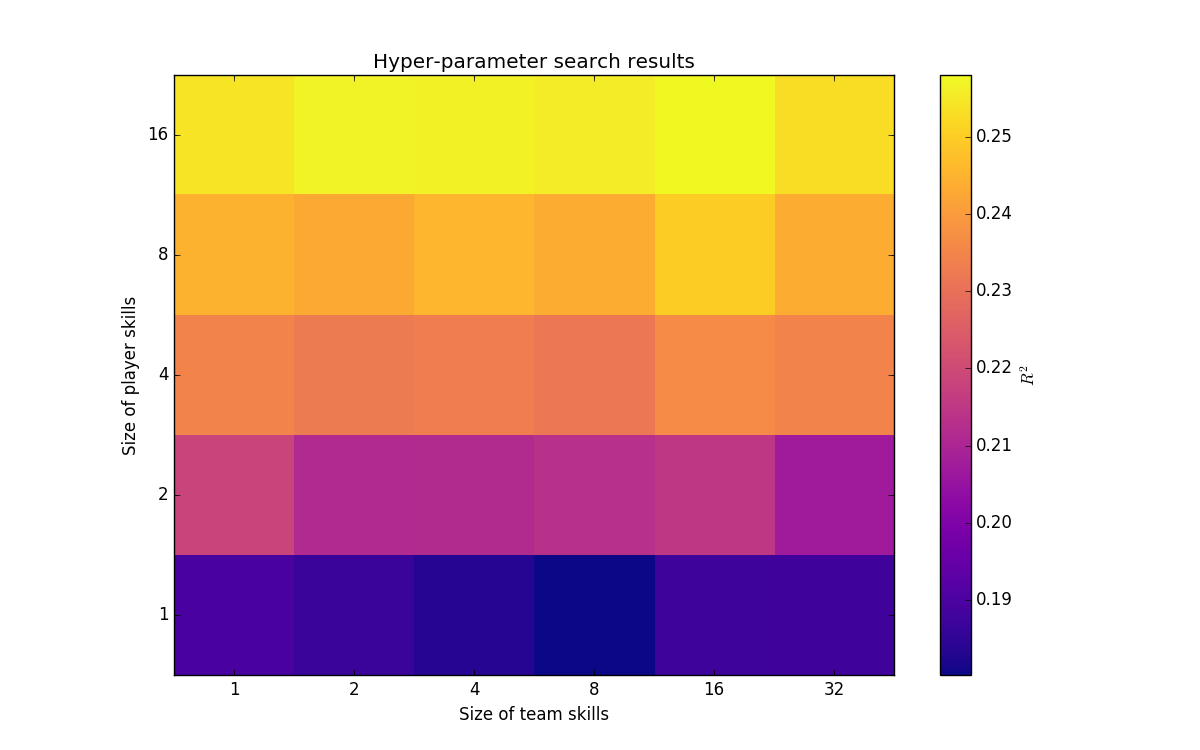
\includegraphics[scale=0.5]{hyper-parameter-search}
\caption{Hyper-parameter search}
\note{As can be seen, increasing the size of player skills has much bigger effect than changing size of team skills.}
\label{fig:hyper-parameter-search}
\end{figure}
The designed model includes three hyper-parameters which have to be adjusted for each game\footnote{There are extra hyper-parameters such as optimisation rate, which are not specific to any game. 
All of the hyper-parameters which I considered are listed in appendix  \ref{hypeparameter-list}.}.
\begin{enumerate}
\item Size of the vector representing player skills.
\item Size of the vector representing team skills.
\item Size and structure of each neural network.
\end{enumerate}
They are ranked in order of importance, adjusting the first should one give the most accuracy increase, but also increase required resources the most.

As can be seen in figure \ref{fig:hyper-parameter-search} the accuracy of the system is mostly dependent on the size of vectors used to represent player skills.
Increasing the size of team skills does not have much of an effect.

This shows the main failure in the model: team skills do not affect the accuracy of the system and therefore I infer that that they are not used by the prediction model.
Therefore the present system does not take into account the skills of other players in the match and only uses the skill of the relevant player.

\paragraph{Learning rate selection}
I have found that varying the learning rate does not have much of an effect on the results of the system.
The only important observation is that since I am using stochastic gradient descent, the system tends to oscillate around the optimum.
The size of such oscillations is determined by the learning rate, higher learning rate leads to bigger oscillations.
Therefore selecting a smaller learning rate usually produces slightly better results, but takes longer to train, although the benefit is not very big.

\section{Performance Evaluation}
The system is designed such there is as little coupling as possible between the two models.
This allowed me to work on each model independently and also made evaluation simpler by allowing me to evaluate both models separately from each other.
\subsection{Prediction model evaluation}
Prediction model is responsible for two functions in the system:
\begin{itemize}
\item Estimating player performance in a particular match
\item Predicting player results given player skills.
\end{itemize}

To evaluate how well different configurations works, pairs of skills and results are taken and split into train/validation parts.
Then the different configurations are trained and validated on the respective parts.
After the results for all configurations are obtained, the best configuration is chosen and used to estimate player performances in each match.
The configuration consists of settings for the five different neural networks from equation \ref{eq:split-conditionals}, namely 
$P(\bs{y}\mid\bs{t})$, $P(\bs{x}_i \mid \bs{t} \bs{p}_i)$, $P(\bs{t} \mid \bs{p})$, $q(\bs{p}_i \mid \bs{t},\bs{x}_i)$, $q(\bs{t}\mid\bs{x},\bs{y})$.

Using hyper-parameter search I discovered that the model functions quite well even without any hidden layers, adding a single hidden layer improves performance a bit.
Increasing the number of hidden layer to two or more gave negligible performance increase and therefore was not used.
Therefore all five neural networks use a simple one hidden layer configuration.
\subsection{Skill update model evaluation}
The accuracy of prediction model depends directly on how accurate the skill estimations of the skill update models are, therefore it is important that skill estimation is as accurate as possible.
To optimise the skill update model, sets of player skills, performances and next performances are taken and then split into train/validation parts.
Skill update model uses only one neural network, $P(\bs{p}_{t+1}\mid\bs{s}_t,\bs{p}_t)$, therefore configuration consists only of the structure of this neural network.
Similarly to prediction model, different configurations are trained and validated and the best is chosen.
The chosen neural network is then used to update the skills of each player at time $t$.

Similarly to neural network in prediction model, neural network without hidden layers worked quite well.
Although in this model, sufficient improvements have been seen in using up to two hidden layers.

\subsection{Overall system evaluation}
To evaluate the system overall co-ordinate descent is performed where prediction model and skill update model are optimised alternatively.
At the start there are no estimates of player skills, therefore the model assumes that all skills are modelled as a standard Gaussian: $\mathcal{N}(0,1)$.
In most cases the optimisation is quite fast only taking two to five rounds of co-ordinate descent.

The co-ordinate descent follows a a simple procedure:
\begin{enumerate}
\item Optimise prediction model and update player performances.
\item Optimise skill update model and update player skills.
\item Validate the whole system.
\item Compare validation result to previous, if it is better save the state of the system and go back to step 1.
If the result is worse, load back the state of the system from last validation and proceed to next step.
\item Test the system using the loaded configuration and report the result.
\end{enumerate}
The system is tested and validated by running the prediction model using the player skill estimates from appropriate time.
Since the system uses cross-validation, steps one, two and three are performed $k$ times, once for each fold of $k$-fold cross-validation.
The validation result in step four is the mean of cross-validation results.

\section{Results}
\subsection{Requirements Satisfaction}
There are five requirements for this project.
Four out of five requirements were satisfied.

Furthermore, as I said in in the subsection \ref{requirements-error}, the original accuracy requirement was not achieved.
If the requirement is interpreted with mistake corrected then the requirement is achieved on one variable.

\paragraph{Predicting the values of different games}
I believe this requirement is satisfied.
I have created a simple game to generate reasonable match results which are different in nature from match results of "Dota 2".
The system was able to predict the match results of my game reasonably well.
Therefore I believe that it will be able to predict match results of most games as long as they are correctly processed and the game itself requires sufficient level of skill.

\paragraph{Prediction based on skills of all players.}
This requirement was not satisfied.
This can be deduced from figure \ref{fig:hyper-parameter-search}, as varying the size of the team skill has little effect on the accuracy of the system.
Further, plugging different values for the skill of other players in the match has little effect on the values predicted for particular player.
Therefore, I concluded that currently the system makes predictions almost exclusively based on the skill of the related player.

This is a biggest failure of the system and would be the first problem that would have to be corrected if the system would be developed further.

\begin{figure}[ht]
\centering
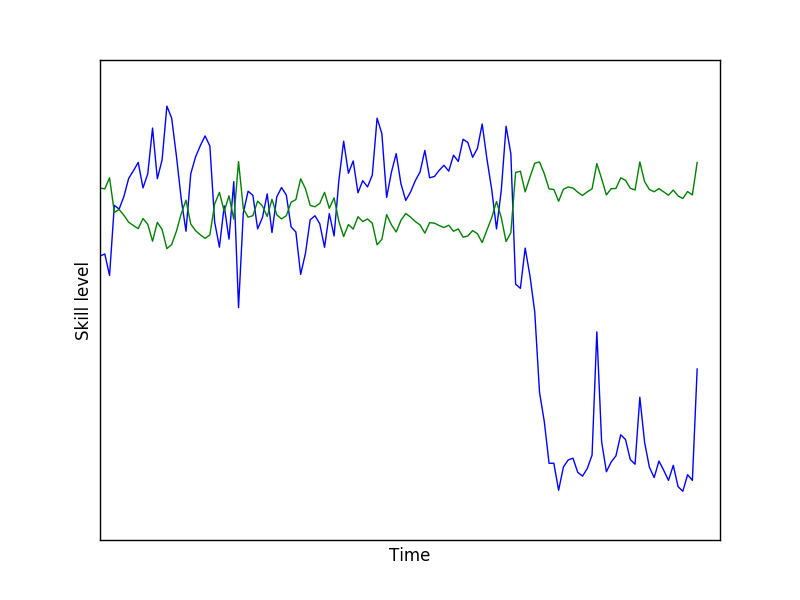
\includegraphics[scale=0.5]{player_skill}
\caption{Change in player's skill through time}
\label{fig:player-skill}
\end{figure}

\paragraph{Time dependent player skill}
This requirement was satisfied.
As can be seen on figure \ref{fig:player-skill}, the magnitude of player's skill varies through time.
Because, these skills are generated using variational inference, I can not tell what each of them represent, therefore they are unlabelled.

\paragraph{Time of execution}
Due to me using approximation by variational methods, the training of the system and prediction times are very small.
Depending on the values of hyper-parameters the training of the system takes between a few minutes and a few hours and prediction in most cases is always extremely quick taking less than a second to predict several hundred match results.
Therefore, I consider this requirement satisfied.

\paragraph{Accuracy and precision of results}
As can be seen in figure \ref{tb:results}, prediction of only one variable has achieved $R^2$ values of more than 0.5, therefore while this requirement was partly satisfied, further work has to be done.
I believe that this requirement is closely linked to the system being able to make predictions based on the skills of all players in the match and if that requirement is satisfied the accuracy and precision of predictions will also greatly improve.

\subsection{Quantitative Results}
\begin{figure}[ht]
\centering
\begin{tabular}{r|r|r|r|r|r|r|r|r}
              & \thead{GPM}   & \thead{XPM}   & \thead{CS}    & \thead{DN}    & \thead{Kills}     & \thead{Deaths}     & \thead{Assists}     & \thead{Level}     \\  \midrule
original $\sigma$          & 0.234 & 0.206 & 0.245 & 0.199 & 0.208 & 0.218 & 0.234 & 0.225 \\ \hline
error $\sigma$   & 0.164 & 0.152 & 0.194 & 0.168 & 0.190 & 0.213 & 0.231 & 0.204 \\ \hline
$R^2$            & \textbf{0.508} & \underline{0.453} & \underline{0.372} & \underline{0.288} & 0.164 & 0.044 & 0.030  & 0.184 \\ \hline
$\sigma$ reduction & 0.299 & 0.260 & 0.208 & 0.156 & 0.086 & 0.022 & 0.015 & 0.097
\end{tabular}
\caption{Quantitative results.}
\note{\emph{GPM} and \emph{XPM} depends mainly on player's playstyle and changes little based on other players in the match, therefore they were predicted well.
While variables such as \emph{kills} and \emph{deaths} depend on player's interaction with the opponents, since the system does not properly account for skills of other players, they are predicted less well.}
\label{tb:results}
\end{figure}
As was expected, different variables were predicted with different levels of success.
The results of predicting the eight main variables\footnote{The explanation of what each variables signifies in game can be found at the end of project proposal in appendix \ref{proposal}} can be seen in figure \ref{tb:results}.

Unfortunately, the accuracy requirement has only been achieved on one variable, I believe this is due to the fact that one of the functional requirements was not achieved.
As the model does not properly take into account the skills of other players, the accuracy suffers.
Furthermore, I believe that such high results were only possible because the teams in most of the matches are fairly matched by the tournament organisers.
If the teams are not well balanced, the effect of skills of other players will have much more of an effect and produce much larger deviations.

\subsection{Baseline comparison to existing systems}
\begin{figure}[ht]
\centering
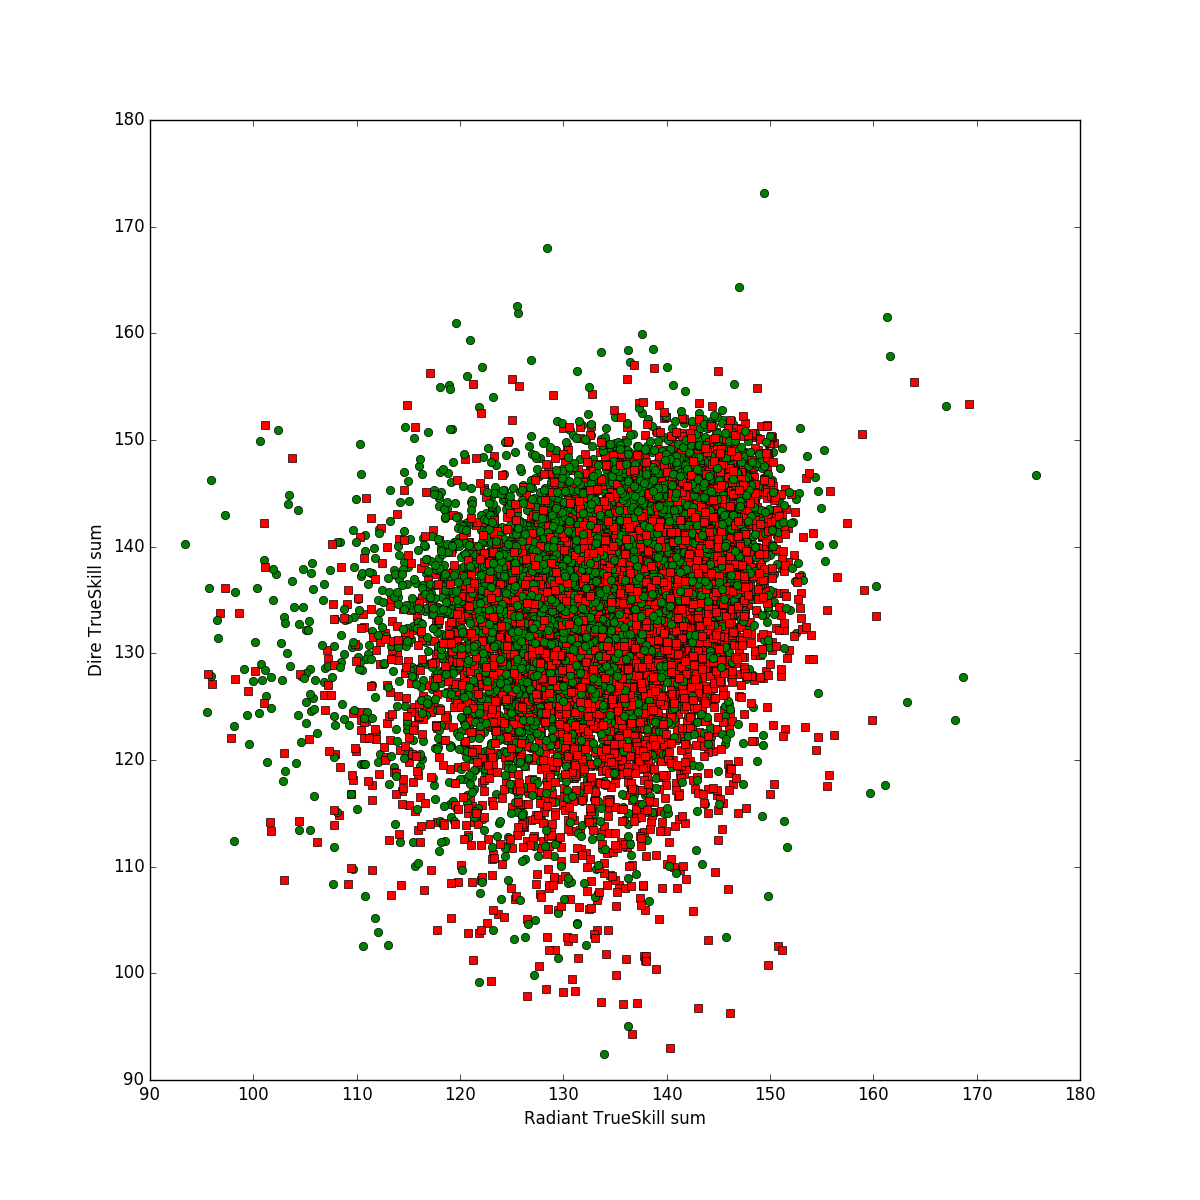
\includegraphics[scale=0.4]{winrate}
\caption{Distribution of skills produced by TrueSkill}
\note{Red points represent matches when Radiant (horizontal axis) team won, while green points represent matches when Dire (vertical axis) team won.}
\label{fig:winrate}
\end{figure}
There do not exist any systems which predict player results in the game, the closest thing that I can use to compare are the rating systems.
TrueSkill is one of the most recent open such systems, I have already used parts of it in my prototype, therefore comparing my system to it required little effort.

TrueSkill library does not directly contain the functionality to predict the outcome of the game, only the probability of a draw.
To make this comparison I made a simple assumption: if the A team's skill calculated by TrueSkill was greater than team B' skill, I assumed that TrueSkill expected team A to win more when playing against team B.
Using this assumption the accuracy of TrueSkill on my dataset was about 0.507.
The graph showing distribution of teams' skills and match outcomes can be seen on figure \ref{fig:winrate}.

My system also does not output the winning team directly, but rather outputs a Bernoulli distribution.
I made a similar assumption, if $p > 0.5$ I assumed team A would win and team B otherwise.
Using this assumption, my system had an accuracy of 0.548, while this is not great, it is much better than TrueSkill accuracy.

\section{Summary}
In this chapter I described how the system was optimised and tested.
The evaluation of the system showed that four out of five requirements have been satisfied and that primary success criteria has been achieved.

\chapter{Conclusions}
\section{Summary of Achievements}
The project has seen reasonable level of success.
Four out of five requirements were satisfied.
The corrected success criteria was achieved on one variable and three other variables were predicted sufficiently well.

The project has shown that using simple methods is not sufficient to accurately predict player results, as the skill of most players changes with time.
By creating a graphical model which can track the skills of the players through time prediction accuracy has been greatly increased.
The graphical model operates on $n$ dimensional vectors and manually determining correct relationships between each value in the vectors was considered impractical.
Instead, neural networks were used to learn such relationships from available data.

The biggest challenge was to decide what each value in the vector of skills should represent.
Since that would require detailed knowledge of the game, variational methods were used to let the model create the interpretation.

\section{Future work and Improvement Ideas}
The biggest problem in the project currently is that the team skills are not used.
I believe that fixing this would increase the accuracy of all predictions, but in particular those that are currently very low.

During the work on this project I had many ideas about how different things can be done and what methods can be used.
Unfortunately, I did not have enough time to try many of them, but I think they should definitely be tested in the future, these include:
\begin{description}
\item[Using Kalman filter for skills updates]
The system represents skills and performances as gaussians, Kalman filter is a perfect candidate for the task.

\item[Using RNN for skill update]
The skill update model treats player performances as observations, therefore using recurrent neural networks with previous $n$ matches as input might produce better results.

\item[Using more results for each match]
The current system only used a very small amount of data available about the game, using more information about each match would definitely improve performance, it would be interesting to know how much.
\end{description}
\section{Lessons Learned}
The main lesson I learned, is not to overestimate my ability when working on novel projects.
While the work done during improvement of an existing feature/product can be hard and challenging, usually the possible improvements can be estimated from similar work, but when working on new idea the results can be much harder to predict since what works in one area might not work in the other.

The second lesson I learned, is that machine learning is not the all-powerful tool that can solve all problems and that most of the time there are still a lot of trade-offs to be made.

\printbibliography[heading=bibintoc,title={Bibliography}]

\appendix
\chapter{Example of a Summary} \label{statexample}
Some parts of this summary are repetitive and take up a lot of space.
In such parts, all but the first set were hidden, indicated by comments.
\begin{minted}[frame=lines,linenos,fontsize=\footnotesize]{json}
{  
   "result":{  
      "players":[  
         {  
            "account_id":87382579,
            "player_slot":0,
            "hero_id":60,
            "item_0":239,
            "item_1":92,
            "item_2":46,
            "item_3":108,
            "item_4":29,
            "item_5":6,
            "backpack_0":0,
            "backpack_1":0,
            "backpack_2":0,
            "kills":3,
            "deaths":7,
            "assists":17,
            "leaver_status":0,
            "last_hits":72,
            "denies":2,
            "gold_per_min":254,
            "xp_per_min":298,
            "level":14,
            "hero_damage":5682,
            "tower_damage":277,
            "hero_healing":170,
            "gold":73,
            "gold_spent":9220,
            "scaled_hero_damage":0,
            "scaled_tower_damage":0,
            "scaled_hero_healing":0,
            "ability_upgrades":[  
               {  
                  "ability":5275,
                  "time":886,
                  "level":1
               },
               "There is one set per level and players can advance up to level 25"
            ]
         },
         "There are nine more sets of player data"
      ],
      "radiant_win":false,
      "duration":2368,
      "pre_game_duration":90,
      "start_time":1471142574,
      "match_id":2569610900,
      "match_seq_num":2244488581,
      "tower_status_radiant":1540,
      "tower_status_dire":1956,
      "barracks_status_radiant":3,
      "barracks_status_dire":63,
      "cluster":113,
      "first_blood_time":89,
      "lobby_type":1,
      "human_players":10,
      "leagueid":4664,
      "positive_votes":38429,
      "negative_votes":2503,
      "game_mode":2,
      "flags":1,
      "engine":1,
      "radiant_score":27,
      "dire_score":30,
      "radiant_team_id":2512249,
      "radiant_name":"Digital Chaos",
      "radiant_logo":692780106202747975,
      "radiant_team_complete":1,
      "dire_team_id":1836806,
      "dire_name":"the wings gaming",
      "dire_logo":352770708597344369,
      "dire_team_complete":1,
      "radiant_captain":87382579,
      "dire_captain":111114687,
      "picks_bans":[  
         {  
            "is_pick":false,
            "hero_id":79,
            "team":1,
            "order":0
         },
         "There are about 20 sets in this list, detailing the drafting phase"
      ]
   }
}
\end{minted}

\chapter{Code for skill update model} \label{code-example}
This as an example of how skill update can be implemented with TensorFlow and Keras.
Implementation of prediction model is similar, but in addition neural networks have to be connected between each other.

\begin{minted}[frame=lines,linenos,fontsize=\footnotesize ,breaklines]{python3}

import keras
import numpy as np
import tensorflow as tf
from keras.layers import Dense


def make_sql_nn(in_dim: int, out_dim: int):
    """
    Create a simple fully-connected, feedforward neural network with two hidden layers.
    """
    p = keras.models.Sequential()
    p.add(Dense(units=int((in_dim + out_dim) * 2 / 3), input_dim=in_dim, activation='relu', kernel_initializer='random_normal'))
    p.add(Dense(units=int((in_dim + out_dim) / 3), activation='relu', kernel_initializer='random_normal'))
    p.add(Dense(units=out_dim, activation='linear', kernel_initializer='random_normal'))
    return p


def log_normal(x, mu, sigma):
    """
    Calculate log of a gaussian pdf.
    """
    error = -(tf.pow((x - mu) / sigma, 2) / 2 + tf.log(tf.clip_by_value(sigma, 1e-8, np.infty)))
    return tf.reduce_sum(error, 1)


def make_mu_and_sigma(nn, tensor):
    """
    Apply neural network to the tensor and then separate the output into parameters for a gaussian distribution.
    """
    mu, log_sigma = tf.split(nn(tensor), num_or_size_splits=2, axis=1)
    sigma = tf.exp(tf.clip_by_value(log_sigma, -5, 5))
    return mu, sigma


PLAYER_DIM = 8

# TensorFlow input variables
player_pre_skill = tf.placeholder(tf.float32, shape=(None, PLAYER_DIM * 2))
player_performance = tf.placeholder(tf.float32, shape=(None, PLAYER_DIM))
player_next_performance = tf.placeholder(tf.float32, shape=(None, PLAYER_DIM))

# Create a neural network
nn = make_sql_nn(PLAYER_DIM + PLAYER_DIM * 2, PLAYER_DIM * 2)

# Apply neural network to input
nn_input = tf.concat([player_pre_skill, player_performance], axis=1)
player_post_skill, sigma = make_mu_and_sigma(nn, nn_input)
log_result = log_normal(player_next_performance, player_post_skill, sigma)

# Save updated skill to a variable
post_skill = tf.concat([player_post_skill, sigma], axis=1)

# Define loss to optimise
loss = -tf.reduce_mean(log_result)
\end{minted}

\chapter{An example of factor graph} \label{factor-graph}
\begin{figure}[h]
\centering
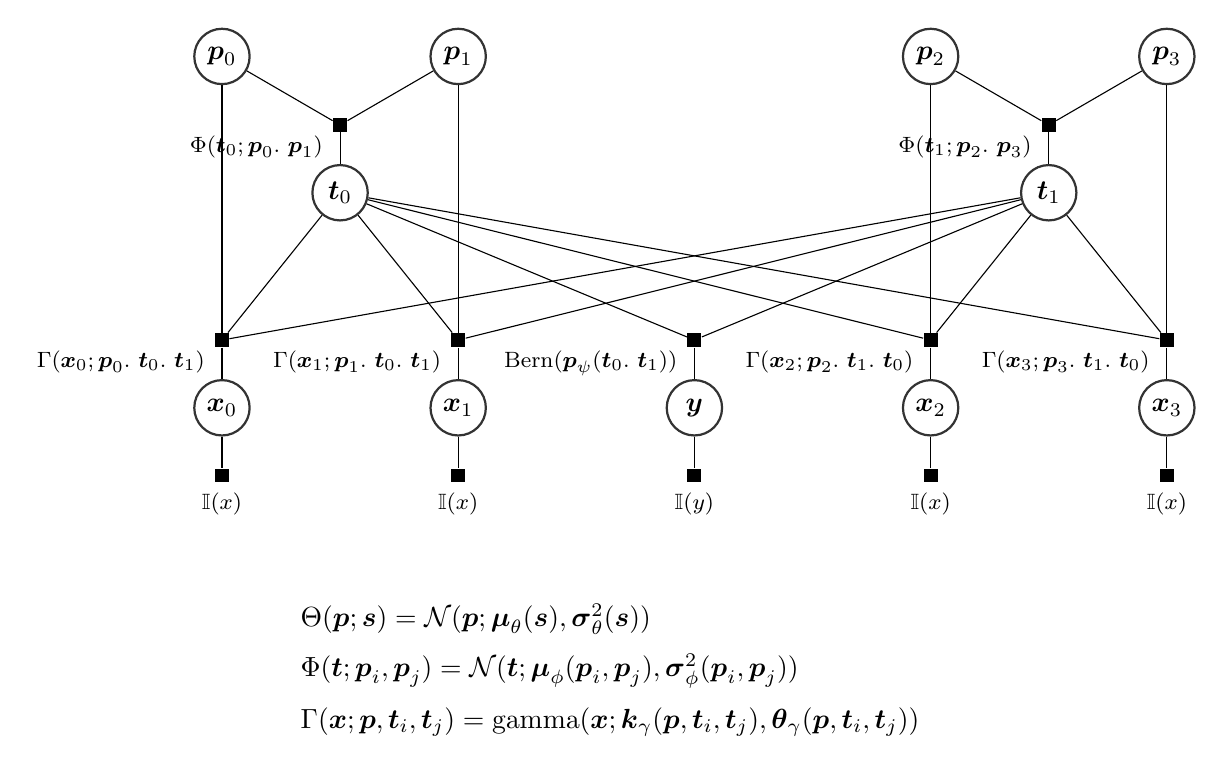
\begin{tikzpicture}
\tikzstyle{main}=[circle, thick, draw=black!80, minimum size=20pt, inner sep=2pt]
\tikzstyle{connect}=[-latex, thick]
\tikzstyle{box}=[rectangle, draw=black!100]
	
	% Team results
	\node[main] (y) [] {$\boldsymbol{y}$};
	
	% Team performances
	\node[main] (t0)[above=2cm of y, xshift=-4.5cm] {$\boldsymbol{t}_0$};
	\node[main] (t1)[above=2cm of y, xshift=4.5cm] {$\boldsymbol{t}_1$};
	
	% Player results
 	\node[main] (x0)[below= 2cm of t0, xshift=-1.5cm] {$\boldsymbol{x}_0$};
 	\node[main] (x1)[below= 2cm of t0, xshift=1.5cm] {$\boldsymbol{x}_1$};
 	\node[main] (x2)[below= 2cm of t1, xshift=-1.5cm] {$\boldsymbol{x}_2$};
 	\node[main] (x3)[below= 2cm of t1, xshift=1.5cm] {$\boldsymbol{x}_3$};
 	
 	% Player performances
 	\node[main] (p0)[above=of t0, xshift=-1.5cm] {$\boldsymbol{p}_0$};
 	\node[main] (p1)[above=of t0, xshift=1.5cm] {$\boldsymbol{p}_1$};
 	\node[main] (p2)[above=of t1, xshift=-1.5cm] {$\boldsymbol{p}_2$};
 	\node[main] (p3)[above=of t1, xshift=1.5cm] {$\boldsymbol{p}_3$};
 	
 	% Player skills
% 	\node[main] (s0)[above=of p0] {$\boldsymbol{s}_0$};
% 	\node[main] (s1)[above=of p1] {$\boldsymbol{s}_1$};
% 	\node[main] (s2)[above=of p2] {$\boldsymbol{s}_2$};
% 	\node[main] (s3)[above=of p3] {$\boldsymbol{s}_3$};
 	
 	% Skill input
% 	\node[factor,label=$\mathcal{N}(\boldsymbol{s}_0;\boldsymbol{\mu}_0.\ \boldsymbol{\sigma}_0^2)$] ()[above=of s0] {}
% 		edge [] (s0);
% 	\node[factor,label=$\mathcal{N}(\boldsymbol{s}_1;\boldsymbol{\mu}_1.\ \boldsymbol{\sigma}_1^2)$] ()[above=of s1] {}
% 		edge [] (s1);
% 	\node[factor,label=$\mathcal{N}(\boldsymbol{s}_2;\boldsymbol{\mu}_2.\ \boldsymbol{\sigma}_2^2)$] ()[above=of s2] {}
% 		edge [] (s2);
% 	\node[factor,label=$\mathcal{N}(\boldsymbol{s}_3;\boldsymbol{\mu}_3.\ \boldsymbol{\sigma}_3^2)$] ()[above=of s3] {}
% 		edge [] (s3);
 		
 	% Skill to performance
% 	\node[factor, label=left:$\Theta(\bs{p}_0;\bs{s}_0)$] () [above=of p0] {}
% 		edge [] (s0)
% 		edge [] (p0);
% 	\node[factor, label=left:$\Theta(\bs{p}_1;\bs{s}_1)$] () [above=of p1] {}
% 		edge [] (s1)
% 		edge [] (p1);
% 	\node[factor, label=left:$\Theta(\bs{p}_2;\bs{s}_2)$] () [above=of p2] {}
% 		edge [] (s2)
% 		edge [] (p2);
% 	\node[factor, label=left:$\Theta(\bs{p}_3;\bs{s}_3)$] () [above=of p3] {}
% 		edge [] (s3)
% 		edge [] (p3);
 		
 	% Performance to team
 	\node[factor, label=185:$\Phi(\bs{t}_0;\bs{p}_0.\ \bs{p}_1)$] () [above=of t0] {}
 		edge [] (p0)
 		edge [] (p1)
 		edge [] (t0);
 	\node[factor, label=185:$\Phi(\bs{t}_1;\bs{p}_2.\ \bs{p}_3)$] () [above=of t1] {}
 		edge [] (p2)
 		edge [] (p3)
 		edge [] (t1);
 		
 	% Team results
 	\node[factor, label=185:$\text{Bern}(\boldsymbol{p}_{\psi}(\boldsymbol{t}_0.\ \boldsymbol{t}_1))$] () [above=of y] {}
 		edge [] (t0)
 		edge [] (t1)
 		edge [] (y);
 	
 	% Player results
 	\node[factor, label=185:$\Gamma(\bs{x}_0;\bs{p}_0.\ \bs{t}_0.\ \bs{t}_1)$] () [above=of x0] {}
 		edge [] (p0)
 		edge [] (t0)
 		edge [] (t1)
 		edge [] (x0);
 	\node[factor, label=185:$\Gamma(\bs{x}_1;\bs{p}_1.\ \bs{t}_0.\ \bs{t}_1)$] () [above=of x1] {}
 		edge [] (p1)
 		edge [] (t0)
 		edge [] (t1)
 		edge [] (x1);
 	\node[factor, label=185:$\Gamma(\bs{x}_2;\bs{p}_2.\ \bs{t}_1.\ \bs{t}_0)$] () [above=of x2] {}
 		edge [] (p2)
 		edge [] (t0)
 		edge [] (t1)
 		edge [] (x2);
 	\node[factor, label=185:$\Gamma(\bs{x}_3;\bs{p}_3.\ \bs{t}_1.\ \bs{t}_0)$] () [above=of x3] {}
 		edge [] (p3)
 		edge [] (t0)
 		edge [] (t1)
 		edge [] (x3);
 		
 	%Results
 	\node[factor,label=below:$\mathbb{I} (x) $] ()[below=of x0] {}
 		edge [] (x0);
 	\node[factor,label=below:$\mathbb{I} (x) $] ()[below=of x1] {}
 		edge [] (x1);
 	\node[factor,label=below:$\mathbb{I} (x) $] ()[below=of x2] {}
 		edge [] (x2);
 	\node[factor,label=below:$\mathbb{I} (x) $] ()[below=of x3] {}
 		edge [] (x3);
	\node[factor,label=below:$\mathbb{I} (y) $] ()[below=of y] {}
 		edge [] (y);
 		
 	\node[text width=10cm] (a0) [below=of y,yshift=-1cm] {$\Theta(\bs{p};\bs{s})=\mathcal{N}(\bs{p};\bs{\mu}_{\theta}(\bs{s}), \bs{\sigma}_{\theta}^2(\bs{s}))$};
 	\node[text width=10cm] (a1) [below=of a0,yshift=1cm] {$\Phi(\bs{t};\bs{p}_i,\bs{p}_j)=\mathcal{N}(\bs{t};\bs{\mu}_{\phi}(\bs{p}_i,\bs{p}_j), \bs{\sigma}_{\phi}^2(\bs{p}_i,\bs{p}_j))$ };
 	\node[text width=10cm] (a2) [below=of a1,yshift=1cm] {
 	$\Gamma(\bs{x};\bs{p},\bs{t}_i,\bs{t}_j)=\text{gamma}(\bs{x};\bs{k}_{\gamma}(\bs{p},\bs{t}_i,\bs{t}_j), \bs{\theta}_{\gamma}(\bs{p},\bs{t}_i,\bs{t}_j))$ };
\end{tikzpicture}
\caption*{This is the factor graph expansion for graphical model in figure \ref{fig:four-player-model}.}
\end{figure}

\chapter{Complete list of system hyper-parameters}\label{hypeparameter-list}
\section{Game-specific hyper-parameters}
The following hyper-parameters have to be adjusted for every game:
\begin{description}
\item[Size of the vector representing player skills] \hfill \\
This depends on complexity of the game and number of variables which the system has to predict.
Games which require a wide variety of skills would require this vector to be bigger, it will also have to be bigger if number of required variables is large.
\item[Size of the vector representing team skills] \hfill \\
This primary depends on the size of the vector representing the player skills as it has to summarise the collective skills of the team.
It also depends on number and variety of roles that can be fulfilled in the game, if all players do the same thing, this will be smaller, if different players try to complete different objectives or play different roles this would have to be bigger.
\item[Period of time to consider during training] \hfill \\
This hyper-parameter depends on how quickly the strategies used by players change and how frequently the rules of the game change.
If the same strategies are used for long periods of time, then much older matches can be considered.
\end{description}

\section{General hyper-parameters}
The following hyper-parameters are related to the system in general:
\begin{enumerate}
\item Optimisation algorithm and parameters of chosen algorithm.
\item Stopping condition for optimisation algorithm.
\end{enumerate}
These are standard machine learning parameters and adjusting them is a complicated task with many possible approaches.

\chapter{Project Proposal}
\label{proposal}

\end{document}
